\documentclass[]{book}
\usepackage{lmodern}
\usepackage{amssymb,amsmath}
\usepackage{ifxetex,ifluatex}
\usepackage{fixltx2e} % provides \textsubscript
\ifnum 0\ifxetex 1\fi\ifluatex 1\fi=0 % if pdftex
  \usepackage[T1]{fontenc}
  \usepackage[utf8]{inputenc}
\else % if luatex or xelatex
  \ifxetex
    \usepackage{mathspec}
  \else
    \usepackage{fontspec}
  \fi
  \defaultfontfeatures{Ligatures=TeX,Scale=MatchLowercase}
\fi
% use upquote if available, for straight quotes in verbatim environments
\IfFileExists{upquote.sty}{\usepackage{upquote}}{}
% use microtype if available
\IfFileExists{microtype.sty}{%
\usepackage{microtype}
\UseMicrotypeSet[protrusion]{basicmath} % disable protrusion for tt fonts
}{}
\usepackage[margin=1in]{geometry}
\usepackage{hyperref}
\hypersetup{unicode=true,
            pdftitle={An Introduction To R},
            pdfauthor={Stuart Hertzog},
            pdfborder={0 0 0},
            breaklinks=true}
\urlstyle{same}  % don't use monospace font for urls
\usepackage{natbib}
\bibliographystyle{plainnat}
\usepackage{color}
\usepackage{fancyvrb}
\newcommand{\VerbBar}{|}
\newcommand{\VERB}{\Verb[commandchars=\\\{\}]}
\DefineVerbatimEnvironment{Highlighting}{Verbatim}{commandchars=\\\{\}}
% Add ',fontsize=\small' for more characters per line
\usepackage{framed}
\definecolor{shadecolor}{RGB}{248,248,248}
\newenvironment{Shaded}{\begin{snugshade}}{\end{snugshade}}
\newcommand{\AlertTok}[1]{\textcolor[rgb]{0.94,0.16,0.16}{#1}}
\newcommand{\AnnotationTok}[1]{\textcolor[rgb]{0.56,0.35,0.01}{\textbf{\textit{#1}}}}
\newcommand{\AttributeTok}[1]{\textcolor[rgb]{0.77,0.63,0.00}{#1}}
\newcommand{\BaseNTok}[1]{\textcolor[rgb]{0.00,0.00,0.81}{#1}}
\newcommand{\BuiltInTok}[1]{#1}
\newcommand{\CharTok}[1]{\textcolor[rgb]{0.31,0.60,0.02}{#1}}
\newcommand{\CommentTok}[1]{\textcolor[rgb]{0.56,0.35,0.01}{\textit{#1}}}
\newcommand{\CommentVarTok}[1]{\textcolor[rgb]{0.56,0.35,0.01}{\textbf{\textit{#1}}}}
\newcommand{\ConstantTok}[1]{\textcolor[rgb]{0.00,0.00,0.00}{#1}}
\newcommand{\ControlFlowTok}[1]{\textcolor[rgb]{0.13,0.29,0.53}{\textbf{#1}}}
\newcommand{\DataTypeTok}[1]{\textcolor[rgb]{0.13,0.29,0.53}{#1}}
\newcommand{\DecValTok}[1]{\textcolor[rgb]{0.00,0.00,0.81}{#1}}
\newcommand{\DocumentationTok}[1]{\textcolor[rgb]{0.56,0.35,0.01}{\textbf{\textit{#1}}}}
\newcommand{\ErrorTok}[1]{\textcolor[rgb]{0.64,0.00,0.00}{\textbf{#1}}}
\newcommand{\ExtensionTok}[1]{#1}
\newcommand{\FloatTok}[1]{\textcolor[rgb]{0.00,0.00,0.81}{#1}}
\newcommand{\FunctionTok}[1]{\textcolor[rgb]{0.00,0.00,0.00}{#1}}
\newcommand{\ImportTok}[1]{#1}
\newcommand{\InformationTok}[1]{\textcolor[rgb]{0.56,0.35,0.01}{\textbf{\textit{#1}}}}
\newcommand{\KeywordTok}[1]{\textcolor[rgb]{0.13,0.29,0.53}{\textbf{#1}}}
\newcommand{\NormalTok}[1]{#1}
\newcommand{\OperatorTok}[1]{\textcolor[rgb]{0.81,0.36,0.00}{\textbf{#1}}}
\newcommand{\OtherTok}[1]{\textcolor[rgb]{0.56,0.35,0.01}{#1}}
\newcommand{\PreprocessorTok}[1]{\textcolor[rgb]{0.56,0.35,0.01}{\textit{#1}}}
\newcommand{\RegionMarkerTok}[1]{#1}
\newcommand{\SpecialCharTok}[1]{\textcolor[rgb]{0.00,0.00,0.00}{#1}}
\newcommand{\SpecialStringTok}[1]{\textcolor[rgb]{0.31,0.60,0.02}{#1}}
\newcommand{\StringTok}[1]{\textcolor[rgb]{0.31,0.60,0.02}{#1}}
\newcommand{\VariableTok}[1]{\textcolor[rgb]{0.00,0.00,0.00}{#1}}
\newcommand{\VerbatimStringTok}[1]{\textcolor[rgb]{0.31,0.60,0.02}{#1}}
\newcommand{\WarningTok}[1]{\textcolor[rgb]{0.56,0.35,0.01}{\textbf{\textit{#1}}}}
\usepackage{longtable,booktabs}
\usepackage{graphicx,grffile}
\makeatletter
\def\maxwidth{\ifdim\Gin@nat@width>\linewidth\linewidth\else\Gin@nat@width\fi}
\def\maxheight{\ifdim\Gin@nat@height>\textheight\textheight\else\Gin@nat@height\fi}
\makeatother
% Scale images if necessary, so that they will not overflow the page
% margins by default, and it is still possible to overwrite the defaults
% using explicit options in \includegraphics[width, height, ...]{}
\setkeys{Gin}{width=\maxwidth,height=\maxheight,keepaspectratio}
\IfFileExists{parskip.sty}{%
\usepackage{parskip}
}{% else
\setlength{\parindent}{0pt}
\setlength{\parskip}{6pt plus 2pt minus 1pt}
}
\setlength{\emergencystretch}{3em}  % prevent overfull lines
\providecommand{\tightlist}{%
  \setlength{\itemsep}{0pt}\setlength{\parskip}{0pt}}
\setcounter{secnumdepth}{5}
% Redefines (sub)paragraphs to behave more like sections
\ifx\paragraph\undefined\else
\let\oldparagraph\paragraph
\renewcommand{\paragraph}[1]{\oldparagraph{#1}\mbox{}}
\fi
\ifx\subparagraph\undefined\else
\let\oldsubparagraph\subparagraph
\renewcommand{\subparagraph}[1]{\oldsubparagraph{#1}\mbox{}}
\fi

%%% Use protect on footnotes to avoid problems with footnotes in titles
\let\rmarkdownfootnote\footnote%
\def\footnote{\protect\rmarkdownfootnote}

%%% Change title format to be more compact
\usepackage{titling}

% Create subtitle command for use in maketitle
\newcommand{\subtitle}[1]{
  \posttitle{
    \begin{center}\large#1\end{center}
    }
}

\setlength{\droptitle}{-2em}
  \title{An Introduction To R}
  \pretitle{\vspace{\droptitle}\centering\huge}
  \posttitle{\par}
  \author{Stuart Hertzog}
  \preauthor{\centering\large\emph}
  \postauthor{\par}
  \date{}
  \predate{}\postdate{}

\usepackage{booktabs}
\usepackage{amsthm}
\makeatletter
\def\thm@space@setup{%
  \thm@preskip=8pt plus 2pt minus 4pt
  \thm@postskip=\thm@preskip
}
\makeatother

\usepackage{amsthm}
\newtheorem{theorem}{Theorem}[chapter]
\newtheorem{lemma}{Lemma}[chapter]
\newtheorem{corollary}{Corollary}[chapter]
\newtheorem{proposition}{Proposition}[chapter]
\newtheorem{conjecture}{Conjecture}[chapter]
\theoremstyle{definition}
\newtheorem{definition}{Definition}[chapter]
\theoremstyle{definition}
\newtheorem{example}{Example}[chapter]
\theoremstyle{definition}
\newtheorem{exercise}{Exercise}[chapter]
\theoremstyle{remark}
\newtheorem*{remark}{Remark}
\newtheorem*{solution}{Solution}
\begin{document}
\maketitle

{
\setcounter{tocdepth}{1}
\tableofcontents
}
\hypertarget{preface}{%
\chapter*{Preface}\label{preface}}
\addcontentsline{toc}{chapter}{Preface}

\textbf{This material is my own process of learning the R programming
language. It can be yours, too.}

\textbf{Originally just notes on R, it grew into a series of
presentations} to the
\href{https://www.meetup.com/Victoria-Raspberry-PiMakers-And-Others/}{VicPiMakers
Meetup Group} in \href{https://www.tourismvictoria.com/}{Victoria BC} in
April and May 2018. Each presentation was created in the
\href{https://www.rstudio.com/}{RStudio IDE} as a series of
\href{http://rmarkdown.rstudio.com/}{RMarkdown} documents that were
output to \href{https://en.wikipedia.org/wiki/HTML}{HTML} then
transferred to a Web hosting site by
\href{https://en.wikipedia.org/wiki/File_Transfer_Protocol}{FTP}.

\textbf{This Series has now become what I hope is a useful tool for
learning R}. Instructions for setting up and using it are given in
\href{setup.html}{How To Set Up This Series}.

Good luck with your R learning!

\emph{Stuart Hertzog,\\
Victoria, BC Canada}

\hypertarget{setup}{%
\chapter{Setup}\label{setup}}

\begin{quote}
You will get the most benefit from this Tutorial Series if you set it up
as an RStudio Project and become familiar with the RStudio IDE.
\end{quote}

\hypertarget{requirements}{%
\section{Requirements}\label{requirements}}

\textbf{This series of tutorials on R can be run on the major computer
platforms -- Mac, Linux, and Windows}.

The necessary files are available in a
\href{https://github.com/stuzog/Intro2R.git}{GitHub repository}. To
download and use them you will need these programs installed on your
computer:

\begin{itemize}
\tightlist
\item
  \href{https://www.r-project.org/}{R}
\item
  \href{https://www.rstudio.com/products/rstudio/download/}{RStudio}
\item
  \href{https://git-scm.com/book/en/v2/Getting-Started-Installing-Git}{git}
\end{itemize}

Once these are properly set up, you can proceed to Installation:

\hypertarget{quick-summary}{%
\section{Quick Summary}\label{quick-summary}}

\textbf{The stages of installing this RStudio Project are}:

\begin{enumerate}
\def\labelenumi{\arabic{enumi}.}
\tightlist
\item
  Install \texttt{r} and \texttt{git} on your computer
\item
  Decide where to put the \emph{Project Directory}
\item
  \texttt{cd} into what will be its parent directory
\item
  Clone the project files from GitHub
\item
  Install and open RStudio on your computer
\item
  Create a new RStudio Project in the \emph{Project Directory}
\item
  Install and initialise \texttt{packrat}
\item
  Set up an account on GitHub if you don't have one
\item
  Create a new repository in your GitHub account
\item
  Add it to RStudio as a \emph{Github destination}
\item
  Push the files in your Project Directory to GitHub
\item
  Continue to \href{Part1_R_Data_Science.html}{Part1} of your
  introduction to R
\end{enumerate}

It may look intimidating, but it's fairly easy to work through.

\hypertarget{installation-details}{%
\section{Installation Details}\label{installation-details}}

Carefully follow these instructions, in this order.

\hypertarget{create-the-project-directory}{%
\subsection{Create The Project
Directory}\label{create-the-project-directory}}

\begin{enumerate}
\def\labelenumi{\arabic{enumi}.}
\item
  In your Terminal program, \texttt{cd} into the directory where you
  want to create the new Project. This can be located wherever you want.
  It will be called \texttt{Intro2R}, so there should not be an existing
  directory with the same name in that location.
\item
  Enter the following commands one at a time at the command line in your
  Terminal program. Follow each line by a \texttt{RETURN}:
\end{enumerate}

\begin{verbatim}
git clone https://github.com/stuzog/Intro2R.git
cd Intro2R
ls -al
\end{verbatim}

You should see a listing of the GitHub repository files (with your user
name):

\begin{verbatim}
total 184
drwxr-xr-x   18 (username)  staff    612 18 Apr 09:10 .
drwxr-xr-x@ 149 (username)  staff   5066 18 Apr 09:10 ..
-rw-r--r--    1 (username)  staff      0 18 Apr 09:10 .Rhistory
-rw-r--r--    1 (username)  staff    117 18 Apr 09:10 .Rprofile
drwxr-xr-x   12 (username)  staff    408 18 Apr 09:10 .git
-rw-r--r--    1 (username)  staff     26 18 Apr 09:10 .gitignore
-rw-r--r--    1 (username)  staff    536 18 Apr 09:10 How.Rmd
-rw-r--r--    1 (username)  staff    225 18 Apr 09:10 Intro2R.Rproj
-rw-r--r--    1 (username)  staff  18366 18 Apr 09:10 Part1_R_Data Science.Rmd
-rw-r--r--    1 (username)  staff  13654 18 Apr 09:10 Part2_R_Programming.Rmd
-rw-r--r--    1 (username)  staff   1360 18 Apr 09:10 README.md
-rw-r--r--    1 (username)  staff  12253 18 Apr 09:10 RStudio.Rmd
-rw-r--r--    1 (username)  staff   8000 18 Apr 09:10 RStudio_Ecosystem.Rmd
-rw-r--r--    1 (username)  staff   2071 18 Apr 09:10 R_Learning_Resources.Rmd
-rw-r--r--    1 (username)  staff    817 18 Apr 09:10 _site.yml
drwxr-xr-x   31 (username)  staff   1054 18 Apr 09:10 images
-rw-r--r--    1 (username)  staff   1682 18 Apr 09:10 index.Rmd
-rw-r--r--    1 (username)  staff    687 18 Apr 09:10 intro.css
\end{verbatim}

\hypertarget{make-it-an-rstudio-project}{%
\subsection{Make It An RStudio
Project}\label{make-it-an-rstudio-project}}

\begin{enumerate}
\def\labelenumi{\arabic{enumi}.}
\setcounter{enumi}{2}
\item
  \textbf{Launch RStudio on your computer}. Unless you have used RStudio
  before, you will see a fairly unpopulated RStudio window.
\item
  \textbf{Start a new RStudio project} by clicking on
  \texttt{R\ Projects} in the upper-right corner of the RStudio window,
  or via the \emph{File \textgreater{} New Project\ldots{}} menu item.
  The \emph{Create New Project} window will appear:
\end{enumerate}

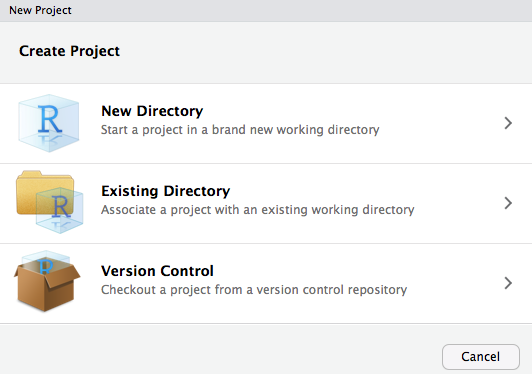
\includegraphics{images/RStudio_new_project_window.png}

\begin{enumerate}
\def\labelenumi{\arabic{enumi}.}
\setcounter{enumi}{4}
\tightlist
\item
  \textbf{Select \emph{Existing Directory}} and navigate to the
  newly-created \texttt{Intro2R} project directory. Click \emph{Open in
  new session} if you wish to preserve the current RStudio session.
\end{enumerate}

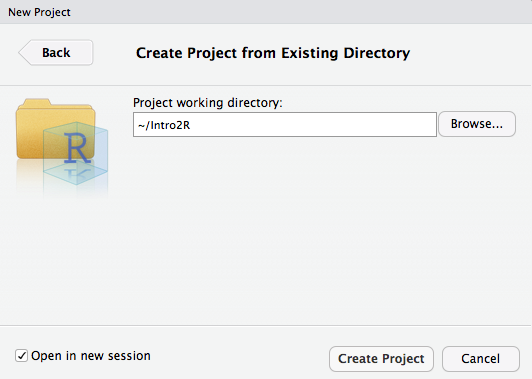
\includegraphics{images/RStudio_create_from_existing_directory_window.png}

\begin{enumerate}
\def\labelenumi{\arabic{enumi}.}
\setcounter{enumi}{5}
\tightlist
\item
  \textbf{Click \emph{Create Project}}. You will see the following
  \texttt{Error} and \texttt{Warning} messages, which you can ignore for
  now. They will be corrected later in the setup.
\end{enumerate}

\begin{verbatim}
Error in file(filename, "r", encoding = encoding) : 
  cannot open the connection
In addition: Warning message:
In file(filename, "r", encoding = encoding) :
  cannot open file 'packrat/init.R': No such file or directory
\end{verbatim}

\hypertarget{install-packrat}{%
\subsection{\texorpdfstring{Install
\texttt{packrat}}{Install packrat}}\label{install-packrat}}

\textbf{Because R packages are updated frequently}, it is recommended
that you use a
\href{http://r.stuzog.com/RStudio.html\#project-package-management}{project
package management} system. This project uses the
\href{https://rstudio.github.io/packrat/}{\texttt{packrat}} package
dependency management system for R, so this should now be installed.

\begin{enumerate}
\def\labelenumi{\arabic{enumi}.}
\setcounter{enumi}{6}
\tightlist
\item
  \textbf{In the \emph{Console window}} at the bottom left of the
  RStudio interface, enter the following commands followed by
  \texttt{RETURN}, one at a time:
\end{enumerate}

\begin{verbatim}
install.packages("packrat")
packrat::init()
\end{verbatim}

The Console will install \texttt{packrat} and the dependencies required
for the project:

\begin{verbatim}
> install.packages("packrat")
Installing package into ‘/Users/(username)/Library/R/3.4/library’
(as ‘lib’ is unspecified)
trying URL 'https://cran.rstudio.com/bin/macosx/el-capitan/contrib/3.4/packrat_0.4.9-1.tgz'
Content type 'application/x-gzip' length 214137 bytes (209 KB)
==================================================
downloaded 209 KB


The downloaded binary packages are in
    /var/folders/qt/6jh4c4yn5zdbf07t61nmz0_w0000gn/T//Rtmptyh6x4/downloaded_packages
> packrat::init()
Initializing packrat project in directory:
- "~/Intro2R"

Adding these packages to packrat:
              _        
    Rcpp        0.12.16
    backports   1.1.2  
    base64enc   0.1-3  
    digest      0.6.15 
    evaluate    0.10.1 
    glue        1.2.0  
    highr       0.6    
    htmltools   0.3.6  
    jsonlite    1.5    
    knitr       1.20   
    magrittr    1.5    
    markdown    0.8    
    mime        0.5    
    packrat     0.4.9-1
    rmarkdown   1.9    
    rprojroot   1.3-2  
    stringi     1.1.7  
    stringr     1.3.0  
    yaml        2.1.18 

Fetching sources for Rcpp (0.12.16) ... OK (CRAN current)
Fetching sources for backports (1.1.2) ... OK (CRAN current)
Fetching sources for base64enc (0.1-3) ... OK (CRAN current)
Fetching sources for digest (0.6.15) ... OK (CRAN current)
Fetching sources for evaluate (0.10.1) ... OK (CRAN current)
Fetching sources for glue (1.2.0) ... OK (CRAN current)
Fetching sources for highr (0.6) ... OK (CRAN current)
Fetching sources for htmltools (0.3.6) ... OK (CRAN current)
Fetching sources for jsonlite (1.5) ... OK (CRAN current)
Fetching sources for knitr (1.20) ... OK (CRAN current)
Fetching sources for magrittr (1.5) ... OK (CRAN current)
Fetching sources for markdown (0.8) ... OK (CRAN current)
Fetching sources for mime (0.5) ... OK (CRAN current)
Fetching sources for packrat (0.4.9-1) ... OK (CRAN current)
Fetching sources for rmarkdown (1.9) ... OK (CRAN current)
Fetching sources for rprojroot (1.3-2) ... OK (CRAN current)
Fetching sources for stringi (1.1.7) ... OK (CRAN current)
Fetching sources for stringr (1.3.0) ... OK (CRAN current)
Fetching sources for yaml (2.1.18) ... OK (CRAN current)
Snapshot written to '/Users/Stuart/Intro2R/packrat/packrat.lock'
Installing Rcpp (0.12.16) ... 
    OK (downloaded binary)
Installing backports (1.1.2) ... 
    OK (downloaded binary)
Installing base64enc (0.1-3) ... 
    OK (downloaded binary)
Installing digest (0.6.15) ... 
    OK (downloaded binary)
Installing glue (1.2.0) ... 
    OK (downloaded binary)
Installing highr (0.6) ... 
    OK (downloaded binary)
Installing jsonlite (1.5) ... 
    OK (downloaded binary)
Installing magrittr (1.5) ... 
    OK (downloaded binary)
Installing mime (0.5) ... 
    OK (downloaded binary)
Installing packrat (0.4.9-1) ... 
    OK (downloaded binary)
Installing stringi (1.1.7) ... 
    OK (downloaded binary)
Installing yaml (2.1.18) ... 
    OK (downloaded binary)
Installing rprojroot (1.3-2) ... 
    OK (downloaded binary)
Installing htmltools (0.3.6) ... 
    OK (downloaded binary)
Installing markdown (0.8) ... 
    OK (downloaded binary)
Installing stringr (1.3.0) ... 
    OK (downloaded binary)
Installing evaluate (0.10.1) ... 
    OK (downloaded binary)
Installing knitr (1.20) ... 
    OK (downloaded binary)
Installing rmarkdown (1.9) ... 
    OK (downloaded binary)
Initialization complete!

Restarting R session...

> 
\end{verbatim}

\begin{enumerate}
\def\labelenumi{\arabic{enumi}.}
\setcounter{enumi}{7}
\tightlist
\item
  \textbf{Click the \emph{Packages tab} in the
  \emph{Files\ldots{}.Viewer pane}} (usually bottom right). It will now
  show a list of packages installed in the Project's dedicated
  \emph{Packrat Library}:
\end{enumerate}

\begin{figure}
\centering
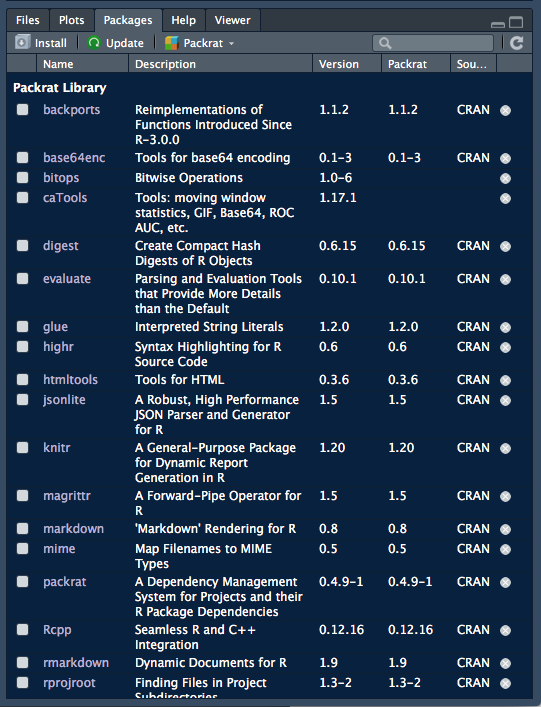
\includegraphics{images/RStudio_packages.png}
\caption{\emph{\textbf{Above:} All Project packages will be installed in
this project-specific library}.}
\end{figure}

\begin{enumerate}
\def\labelenumi{\arabic{enumi}.}
\setcounter{enumi}{8}
\tightlist
\item
  \textbf{Click \emph{Update} in the \emph{Packages tab toolbar}} to
  ensure that all project packages are current. Packages are updated
  frequently, so it is advisable to do this from time to time.
\end{enumerate}

\hypertarget{github-version-control}{%
\section{GitHub Version Control}\label{github-version-control}}

\textbf{It's a really good idea to track your R coding with some form of
\href{https://support.rstudio.com/hc/en-us/articles/200532077-Version-Control-with-Git-and-SVN}{version
control}}.

RStudio makes this easy for you.

\textbf{\href{https://git-scm.com/}{git} and
\href{https://github.com/explore}{GitHub} have become the leading
version control system} --- there's even a
\href{https://git-scm.com/book/en/v2}{free eBook} about \texttt{git}
available for download . There also are some
\href{https://r-bio.github.io/intro-git-rstudio/}{easy-to-understand
explanations} on how \texttt{git} works available on the Web.

\textbf{\texttt{git} support is built-in to RStudio}. This makes keeping
track of your many ch-ch-ch-changes an integral part of your R
programming workflow.

\hypertarget{setting-up-git-in-rstudio}{%
\subsection{\texorpdfstring{Setting Up \texttt{git} In
RStudio}{Setting Up git In RStudio}}\label{setting-up-git-in-rstudio}}

How you set up \texttt{git} in RStudio depends on whether you are:

\begin{itemize}
\tightlist
\item
  \textbf{Starting a new Project}:

  \begin{itemize}
  \tightlist
  \item
    \href{http://happygitwithr.com/new-github-first.html}{first from
    GitHub}
  \item
    \href{https://support.rstudio.com/hc/en-us/articles/200532077-Version-Control-with-Git-and-SVN}{from
    RStudio}
  \item
    \href{http://happygitwithr.com/clone.html}{from a GitHub clone}
  \end{itemize}
\item
  \textbf{Adding \texttt{git} to an existing Project}

  \begin{itemize}
  \tightlist
  \item
    \href{http://happygitwithr.com/existing-github-first.html}{starting
    from GitHub}, or
  \item
    \href{http://happygitwithr.com/existing-github-last.html}{starting
    from RStudio}
  \end{itemize}
\end{itemize}

Each alternative takes a slightly different path through the
RStudio/GitHub maze. They are best detailed in
\href{http://happygitwithr.com/}{Happy Git and GitHub for the useR} by
Jenny Bryan and the STAT 545 Teaching Assistants of UBC.
\href{https://support.rstudio.com/hc/en-us/articles/200532077-Version-Control-with-Git-and-SVN}{RStudio's
version control guide} also shows how to use \texttt{git} or an
\href{http://subversion.apache.org/}{SVN repository} for version
control.

\hypertarget{using-git-in-rstudio}{%
\subsection{\texorpdfstring{Using \texttt{git} In
RStudio}{Using git In RStudio}}\label{using-git-in-rstudio}}

\textbf{When \texttt{git} is properly set up, a new \emph{Git} tab} will
appear in the \emph{Environment\ldots{} Build} pane. Clicking on this
tab will show files and directories that have changed since the last
synchronisation with the \emph{GitHub repository} associated with this
Project. If you keep this tab open, you will see its contents change
each time you save a file, or rebuild an entire Web site.

\begin{figure}
\centering
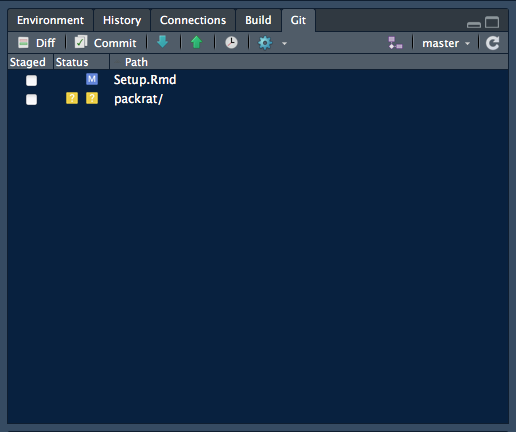
\includegraphics{images/RStudio_git_pane.png}
\caption{\emph{\textbf{Above:} The Git pane showing changes during work
on this .Rmd file}}
\end{figure}

\textbf{The \emph{GitHub Push} workflow is}:

\begin{enumerate}
\def\labelenumi{\arabic{enumi}.}
\tightlist
\item
  \emph{Stage} any modified file or directory
\item
  \emph{Commit} selected \emph{Staged} files or directories, adding a
  brief \emph{Commit message}
\item
  \emph{Push} all \emph{Committed} files/directories to a \emph{GitHub
  repository}.
\end{enumerate}

\textbf{If you're new to \texttt{git} and somewhat intimidated by it},
\href{https://medium.com/@ashk3l/a-visual-introduction-to-git-9fdca5d3b43a}{A
Visual Introduction to Git} gives an amusing introduction to the basic
\texttt{git} workflow.

\textbf{For a detailed overview from a developer perspective} see
\href{http://r-pkgs.had.co.nz/git.html}{Git and GitHub} by Hadley
Wickham. It particulaly refers to R package development.

\hypertarget{staging-changed-items}{%
\subsubsection{Staging Changed Items}\label{staging-changed-items}}

\begin{enumerate}
\def\labelenumi{\arabic{enumi}.}
\item
  \textbf{Click its \emph{Staged} checkbox}
  
\includegraphics{images/git-blank-button.png} A small blue box
  
\includegraphics{images/git-blue-M.png} appears in the left
  \emph{Status} column, showing that the file or directory was
  \emph{Modified} and ready for a \emph{Commit}. If you had only added
  the file, a small green box 
\includegraphics{images/git-green-A.png}
  will appear. The \emph{Staged} checkbox then changes to a tickmark
  
\includegraphics{images/git-check-button.png}.
\item
  \textbf{If you click on a listed directory}, its contents will all
  appear, marked \emph{Staged} and with small green boxes
  
\includegraphics{images/git-green-A.png} signifying that they have
  been \emph{Added.}
\end{enumerate}

\begin{figure}
\centering
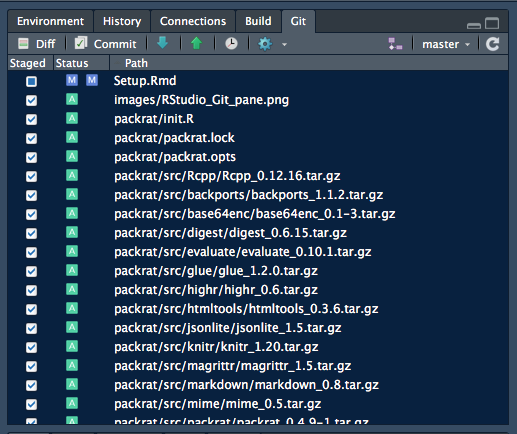
\includegraphics{images/RStudio_staged_directories.png}
\caption{\emph{\textbf{Above:} Staging a directory will result in its
contents all being shown Staged.}}
\end{figure}

\begin{enumerate}
\def\labelenumi{\arabic{enumi}.}
\setcounter{enumi}{2}
\tightlist
\item
  \textbf{To \emph{Unstage} added sub-directories or files} you either
  deselect each individually then deselect the \emph{Staged} parent
  directory (\emph{Tip:} Start with the bottom one and keep clicking!),
  or \texttt{SHIFT\ Click} all of them and uncheck one \emph{Selected}
  radio button.
\end{enumerate}

\hypertarget{those-little-git-icons}{%
\subsubsection{\texorpdfstring{Those little \texttt{git}
icons?}{Those little git icons?}}\label{those-little-git-icons}}

In the \emph{Status} column, you'll see little yellow, blue, or red
icons. They mean:


\includegraphics{images/git-yellow-N.png} - \emph{New file} or directory
that does not exist in the \texttt{git} \emph{Repository}\\

\includegraphics{images/git-blue-M.png} - \emph{Modified} from what is
in the \texttt{git} \emph{Repository}\\

\includegraphics{images/git-green-A.png} - \emph{Staging} a file or
adding it to be committed\\

\includegraphics{images/git-red-D.png} - The item has been
\emph{Deleted}

The \emph{Status} column has a \emph{left} and \emph{right} icon
alignment:

\emph{icon on the left} - the item has been \emph{Staged}\\
\emph{icon on the right} - the item is \emph{Not Staged}

Sometimes you'll see icons in both columns:


\includegraphics{images/git-yellow-N.png}

\includegraphics{images/git-yellow-N.png} - \emph{Not in the Repository}
and has changed recently\\

\includegraphics{images/git-blue-M.png}

\includegraphics{images/git-blue-M.png} - \emph{Staged} and
\emph{Modified} since it was \emph{Staged}

In the last case, the \emph{Staged} checkbox will be filled with a solid
blue 
\includegraphics{images/git-blue-button.png}.

You'll see how it all works as you continue with RStudio.

\hypertarget{committing-staged-items}{%
\subsubsection{Committing Staged Items}\label{committing-staged-items}}

When you have \emph{Staged} everything you want, the next step is to
\emph{Commit} those \emph{Staged} items.

\begin{enumerate}
\def\labelenumi{\arabic{enumi}.}
\setcounter{enumi}{3}
\tightlist
\item
  \textbf{Click the \emph{Commit} button to do this}. The \emph{Review
  Changes} window appears. You can add a message to remind you (and
  others) what you have done in this \emph{Commit}. This is always
  advisable, especially for others reviewing your repository.
\end{enumerate}

\begin{figure}
\centering
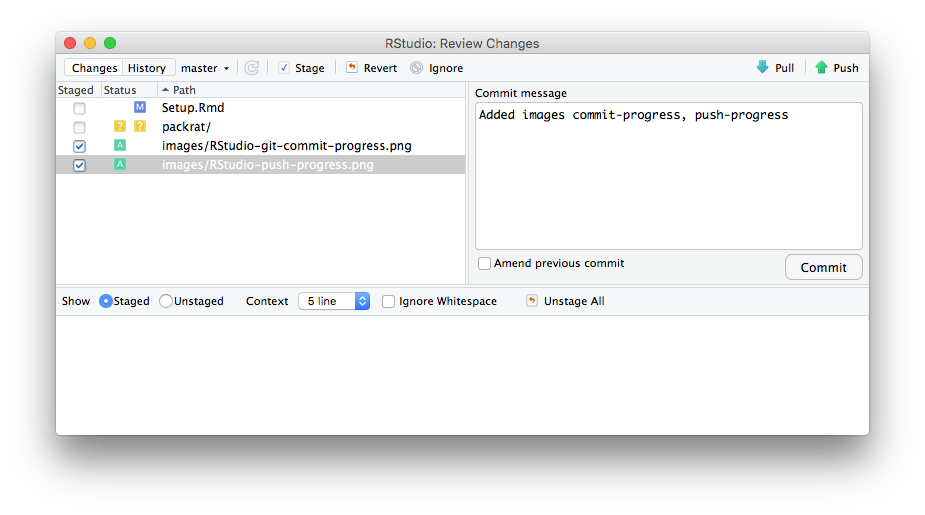
\includegraphics{images/RStudio-review-changes.png}
\caption{\emph{\textbf{Above:} The RStudio Review Changes window with a
Commit message.}}
\end{figure}

A smaller \emph{Progress window} will open over the \emph{Review
window}. It is actually a small \emph{Terminal window} showing what you
would see if you were at the command line.

\begin{figure}
\centering
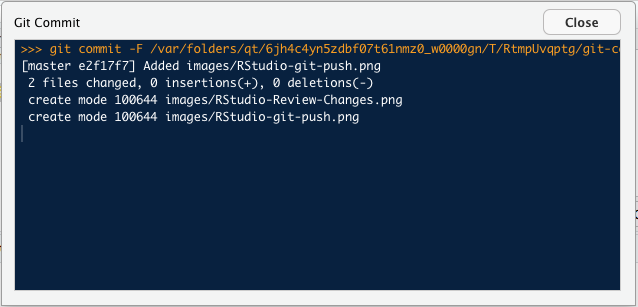
\includegraphics{images/RStudio-git-commit-progress.png}
\caption{\emph{\textbf{Above:} The Progress window shows the result of
your Commit command.}}
\end{figure}

\hypertarget{pushing-to-github}{%
\subsubsection{Pushing To GitHub}\label{pushing-to-github}}

\begin{enumerate}
\def\labelenumi{\arabic{enumi}.}
\setcounter{enumi}{4}
\tightlist
\item
  Your files are now Committed; the next step is to \textbf{Push} them
  to the Repository. The \texttt{green\ up-arrow} is the \textbf{Push
  button}. You may have to close the \emph{Progress window} first.
\end{enumerate}

\begin{figure}
\centering
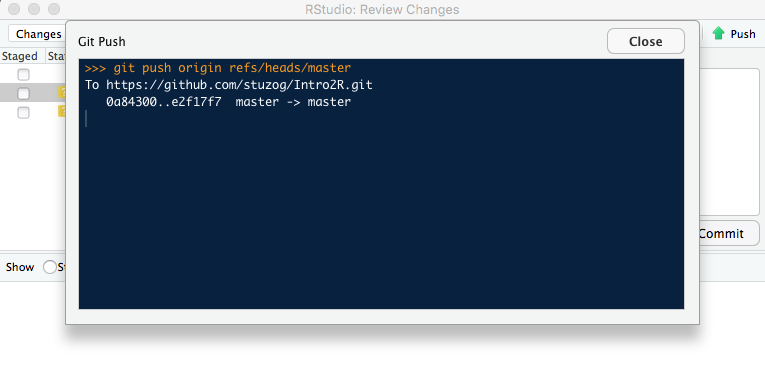
\includegraphics{images/RStudio-push-progress.png}
\caption{\emph{\textbf{Above:} The Push only happens when you click the
green Push button.}}
\end{figure}

\begin{enumerate}
\def\labelenumi{\arabic{enumi}.}
\setcounter{enumi}{5}
\tightlist
\item
  If everything went well, you will see the above message in the
  \emph{Progress window} (opens automatically if you had closed it).
\end{enumerate}

\begin{figure}
\centering
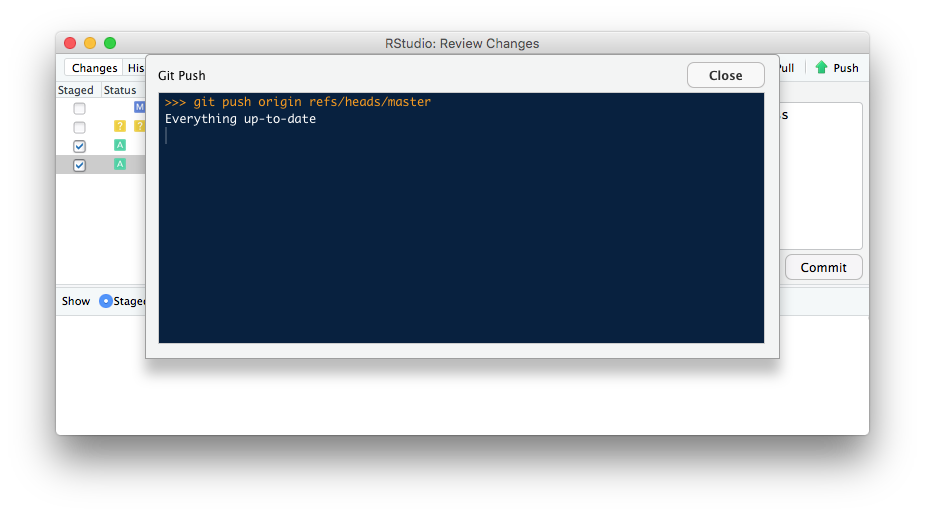
\includegraphics{images/RStudio-push-changes.png}
\caption{\emph{\textbf{Above:} After a successful Push, a second Push
shows everything up-to-date.}}
\end{figure}

\hypertarget{r-for-data-science}{%
\chapter{R For Data Science}\label{r-for-data-science}}

\begin{quote}
``In Data Science there's always a human in the loop: someone is
understanding the insight, seeing the figure, or benefitting from the
conclusion.'' ---
\href{http://varianceexplained.org/r/ds-ml-ai/}{\emph{David Robinson,
Variance Explained Blog}}
\end{quote}

That person can be called a \textbf{Data Scientist}.

\hypertarget{what-is-data-science}{%
\section{What Is Data Science?}\label{what-is-data-science}}

\begin{itemize}
\item
  \href{https://en.wikipedia.org/wiki/Data_science}{Data Science} is a
  discipline that uses \emph{statistics, data analysis, machine
  learning} and their \emph{related methods} to \textbf{understand and
  analyze actual phenomena}.
\item
  It employs techniques and theories of \textbf{mathematics, statistics,
  information science}, and \textbf{computer science}, in particular the
  subdomains of \emph{machine learning, classification, cluster
  analysis, uncertainty quantification, computational science, data
  mining, databases,} and \emph{visualization}.
\end{itemize}

According to Wikipedia:

\begin{itemize}
\item
  \href{https://en.wikipedia.org/wiki/Data_analysis}{Data Analysis} is a
  \textbf{descriptive process} of inspecting, cleansing, transforming,
  and modeling data with the goal of \textbf{discovering useful
  information, suggesting conclusions}, and \textbf{supporting
  decision-making}.
\item
  \href{https://en.wikipedia.org/wiki/Data_mining}{Data Mining} is a
  particular data analysis technique for \textbf{discovering patterns in
  large data sets}. It focuses on modeling and knowledge discovery for
  \textbf{predictive} rather than purely \textbf{descriptive} purposes.
\item
  \href{https://en.wikipedia.org/wiki/Data_modeling}{Data Modeling} is a
  process used to define and analyze the \textbf{data requirements
  needed to support business processes} within \textbf{information
  systems in organizations}.
\item
  \href{https://en.wikipedia.org/wiki/Business_intelligence}{Business
  Intelligence} comprises the strategies and technologies used by
  enterprises for the \textbf{data analysis of business information} to
  provide historical, current and predictive views of \textbf{business
  operations}.
\end{itemize}

\textbf{R is used in two associated disciplines}, which are often
confused as also being Data Science:

\begin{itemize}
\item
  \href{https://en.wikipedia.org/wiki/Machine_learning}{Machine
  Learning} (ML) gives computer systems the ability to
  \textbf{progressively improve performance of a specific task} with
  data, without being explicitly programmed, and
\item
  \href{https://en.wikipedia.org/wiki/Artificial_intelligence}{Artificial
  Intelligence} (AI), in contrast to the natural intelligence displayed
  by humans and other animals, is intelligence demonstrated by machines
  through \textbf{Intelligent Agents} that \textbf{perceive their
  environment} and \textbf{take actions} to maximize the chance of
  successfully achieving their designers' intended goals.
\end{itemize}

\textbf{Although they overlap}, Data Science, Machine Learning, and
Artificial Intelligence produce different outcomes:

\begin{itemize}
\tightlist
\item
  \textbf{Data Science} produces \emph{\textbf{insights}}
\item
  \textbf{Machine Learning} produces \emph{\textbf{prediction}s}
\item
  \textbf{Artificial Intelligence} produces \emph{\textbf{actions}}
\end{itemize}

\hypertarget{what-is-r}{%
\section{What Is R?}\label{what-is-r}}

\begin{quote}
R is a functional programming language designed to manipulate, display,
and analyse statistical data.
\end{quote}

R is a \textbf{free, case-sensitive, interpreted} language that uses
statistical techniques \textbf{to perform}
\href{https://en.wikipedia.org/wiki/Data_analysis}{Data Analysis},
\href{https://en.wikipedia.org/wiki/Data_mining}{Data Mining},
\href{https://en.wikipedia.org/wiki/Data_modeling}{Data Modeling}, and
\href{https://en.wikipedia.org/wiki/Machine_learning}{Machine Learning},
\textbf{and to create}
\href{https://www.innoarchitech.com/python-vs-or-r-artificial-intelligence-ai-machine-learning-data-science-which-use/}{Artifical
Intelligence} and
\href{https://en.wikipedia.org/wiki/Business_intelligence}{Business
Intelligence}.

\begin{itemize}
\tightlist
\item
  R is a \textbf{functional programming language}, not
  \textbf{procedural}.
\item
  It is \textbf{vector-based} and \textbf{highly-optimised} to speedily
  and efficiently manipulate and display all types of \textbf{numeric}
  and \textbf{graphical} data.
\item
  R \textbf{holds data in memory} for speedy access, so it runs

  \begin{itemize}
  \tightlist
  \item
    \textbf{better on fast processors} with lots of memory for
    \textbf{large datasets}
  \item
    but can be run on an \textbf{distributed cluster} running
    \href{https://hadoop.apache.org/}{Apache Hadoop}, either
  \item
    on a \textbf{local network} or on a
    \textbf{\href{https://www.technavio.com/blog/top-16-companies-in-the-hadoop-as-a-service-hdaas-market}{Hadoop
    cloud service}}.
  \end{itemize}
\item
  R was \textbf{developed from
  \href{https://en.wikipedia.org/wiki/S_(programming_language)}{S}},
  which was \textbf{created in 1976} by
  \textbf{\href{https://en.wikipedia.org/wiki/John_Chambers_(statistician)}{John
  Chambers}} of
  \textbf{\href{https://en.wikipedia.org/wiki/Bell_Labs}{Bell Labs}}.
\item
  It was \textbf{written by
  \href{https://en.wikipedia.org/wiki/Ross_Ihaka}{Ross Ihaka} and
  \href{https://en.wikipedia.org/wiki/Robert_Gentleman_(statistician)}{Robert
  Gentleman}} at the
  \textbf{\href{https://en.wikipedia.org/wiki/University_of_Auckland}{University
  of Auckland}}, New Zealand.
\item
  The name R comes partly from the names of the two authors, and partly
  as a play on S.
\item
  R was \textbf{conceived in 1992} with an initial version released in
  \textbf{1995}, and a stable beta version in \textbf{2000}.
\item
  While there are some important differences, most \textbf{S code can
  run unaltered in R}.
\item
  R is currently being actively developed by the
  \textbf{\href{https://www.r-project.org/contributors.html}{R
  Development Core Team}}, which includes John Chambers.
\item
  Development of R is supported by the
  \textbf{\href{https://www.r-project.org/}{R Project for Statistical
  Computing}}.
\item
  R is freely available under the
  \textbf{\href{https://www.gnu.org/licenses/gpl-3.0.en.html}{GNU
  General Public License}}. Pre-compiled binary versions are provided
  for various operating systems. These are available on \textbf{local
  \href{https://cran.r-project.org/mirrors.html}{CRAN mirrors}}.
\end{itemize}

\begin{quote}
The source code for the R software environment is written primarily in
\textbf{C, Fortran, and R}, highly-optimised for fast computation of
large collections of statistical data.
\end{quote}

The \textbf{popularity of R has increased substantially} in recent
years. As of March 2018, R is \textbf{in the top 20 of the
\href{https://www.tiobe.com/tiobe-index/}{TIOBE index}}, (Python was
ranked \#4 at that time).

\hypertarget{installing-r}{%
\section{Installing R}\label{installing-r}}

\textbf{R must be installed} on a computer as currently it is
\textbf{not included} in any operating system. Precompiled versions are
available for major systems including \textbf{Windows}, \textbf{MacOS},
and \textbf{Linux}. It may \textbf{require compiling} on some Linux
distributions.

R is available from the \href{https://cran.r-project.org/}{Comprehensive
R Archive Network (CRAN)}, via a multinational network of
\href{https://cran.r-project.org/mirrors.html}{CRAN Mirrors}.
\textbf{Canadian CRAN mirrors} are hosted at:

\begin{itemize}
\tightlist
\item
  \href{http://cran.stat.sfu.ca/}{Simon Fraser University}
\item
  \href{http://muug.ca/mirror/cran/}{Manitoba Unix User Group}
\item
  \href{http://cran.utstat.utoronto.ca/}{University of Toronto}
\item
  \href{http://mirror.its.dal.ca/cran/}{Dalhousie University}
\end{itemize}

\textbf{Precompiled versions} are available for:

\begin{itemize}
\tightlist
\item
  \href{http://cran.stat.sfu.ca/bin/linux/}{Download for Linux} (SFU)
\item
  \href{http://cran.stat.sfu.ca/bin/macosx/}{Download for OS X} (SFU)
\item
  \href{http://cran.stat.sfu.ca/bin/windows/}{Download for Windows}
  (SFU)
\end{itemize}

\hypertarget{command-line-r}{%
\section{Command Line R}\label{command-line-r}}

R can be run from the command line in a Terminal window:

\begin{itemize}
\tightlist
\item
  \texttt{which\ R} -- find the location of the R executable
\item
  \texttt{R\ -\/-version} -- show the currently installed version of R
\item
  \texttt{R} -- start an interactive R session
\end{itemize}

Version information is shown (as above) and the R command prompt
\texttt{\textgreater{}} is available.

\begin{itemize}
\tightlist
\item
  \texttt{quit()} -- quit an R session**
\end{itemize}

\hypertarget{help-and-manuals}{%
\subsection{Help and Manuals}\label{help-and-manuals}}

\begin{itemize}
\item
  Help is available in the usual way with \texttt{R\ -\/-help}
\item
  \href{https://cran.r-project.org/manuals.html}{Downloadable manuals
  for R} are available in \textbf{HTML}, \textbf{PDF}, and \textbf{EPUB}
  formats.
\item
  The \textbf{LaTeX or Texinfo sources} of the latest version of these
  documents are contained in every R source distribution, in the
  subdirectory \texttt{doc/manual} of the extracted archive.
\item
  The \textbf{HTML versions of the manuals} are also part of most R
  installations, accessible by entering the function
  \texttt{help.start()} at the R prompt to launch a page in your default
  Web browser with links to local R documentation.
\item
  \textbf{Manuals for older R versions} are available in the
  \href{https://cran.r-project.org/src/base/}{archives of the R
  sources}.
\end{itemize}

\hypertarget{the-r-console-interface}{%
\section{The R Console Interface}\label{the-r-console-interface}}

While R has a command line interface, a graphical interface is installed
as an executable application \texttt{R.app} or \texttt{R.exe} for
\textbf{Windows}, \textbf{MacOS}, and \textbf{Linux}. With minor
platform differences, they are similar to this startup screen on
\textbf{OS X}:

\begin{figure}
\centering
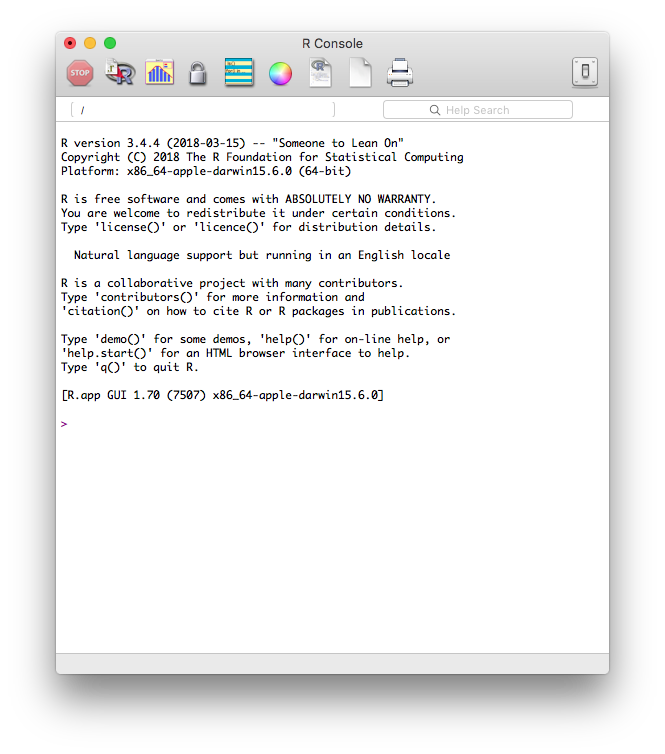
\includegraphics{images/R_Console.png}
\caption{\emph{\textbf{Above:} The R Console startup screen in OS X
10.11.6 El Capitan}}
\end{figure}

R commands can be \textbf{run from the command prompt} in R Console,
similar to using the \textbf{command line interface} in a terminal
program.

\hypertarget{access-to-r-help}{%
\subsection{Access To R Help}\label{access-to-r-help}}

\textbf{Tooltip help} appears on hovering the cursor over the
\textbf{icons in the Toolbar} along the top of the Console window.
\textbf{Access to R Help files} is invoked by entering
\texttt{help.start()} at the command prompt. This will launch the
\textbf{R Help server} on your computer and open a \textbf{comprehensive
Help page} in your Web browser.

\begin{verbatim}
> help.start()
starting httpd help server ... done
If the browser launched by '/usr/bin/open' is already running, it is
    *not* restarted, and you must switch to its window.
Otherwise, be patient ...
> 
\end{verbatim}

\begin{figure}
\centering
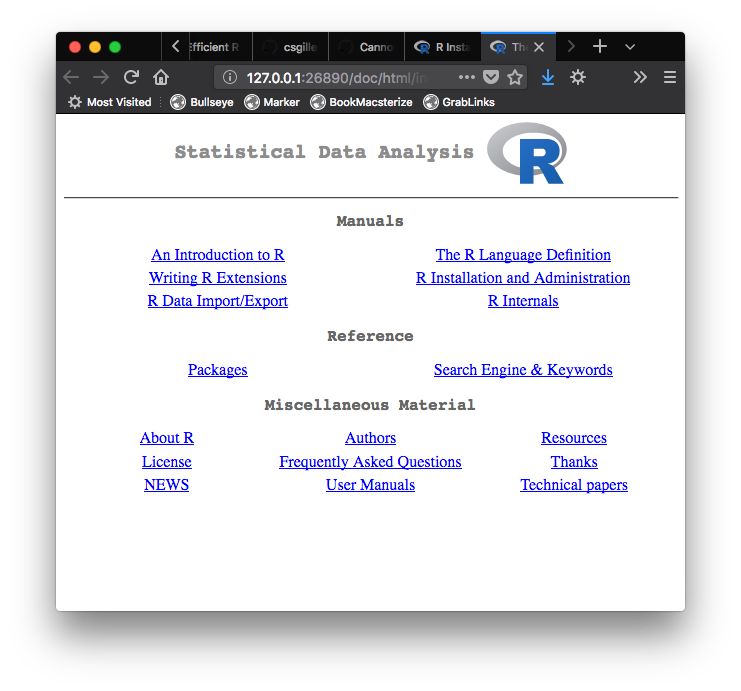
\includegraphics{images/R_Help.png}
\caption{\emph{\textbf{Above:} The R Language Help page opens in your
default Web browser}}
\end{figure}

\hypertarget{data-file-management}{%
\subsection{Data File Management}\label{data-file-management}}

An R installation includes a treasure-trove of \textbf{statistical data
files}. These can be seen using the \textbf{Data Manager}, available
under the \emph{Packages \& Data} menu. Clicking on a dataset will
display its \textbf{documentation in the lower pane} of the R Data
Manager.

\begin{figure}
\centering
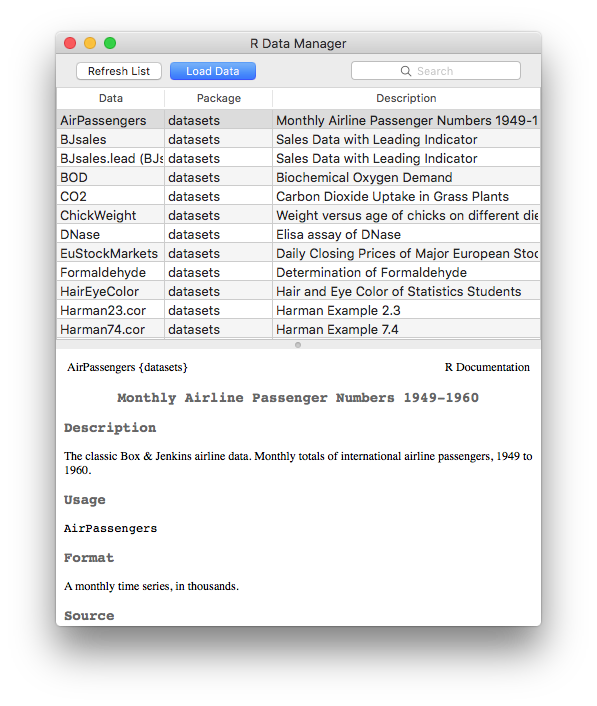
\includegraphics{images/R_Data_Manager.png}
\caption{\emph{\textbf{Above:} The Data Manager lists the extensive
statistical datasets included with R.}}
\end{figure}

\hypertarget{package-management}{%
\subsection{Package Management}\label{package-management}}

\textbf{R Console has a built-in Package Management system} that can be
invoked from the \textbf{Packages \& Data} menu. The top pane of the
\textbf{R Package Manager} window lists all installed packages. Clicking
on a package brings up its \textbf{Documentation} in the lower window.

\begin{figure}
\centering
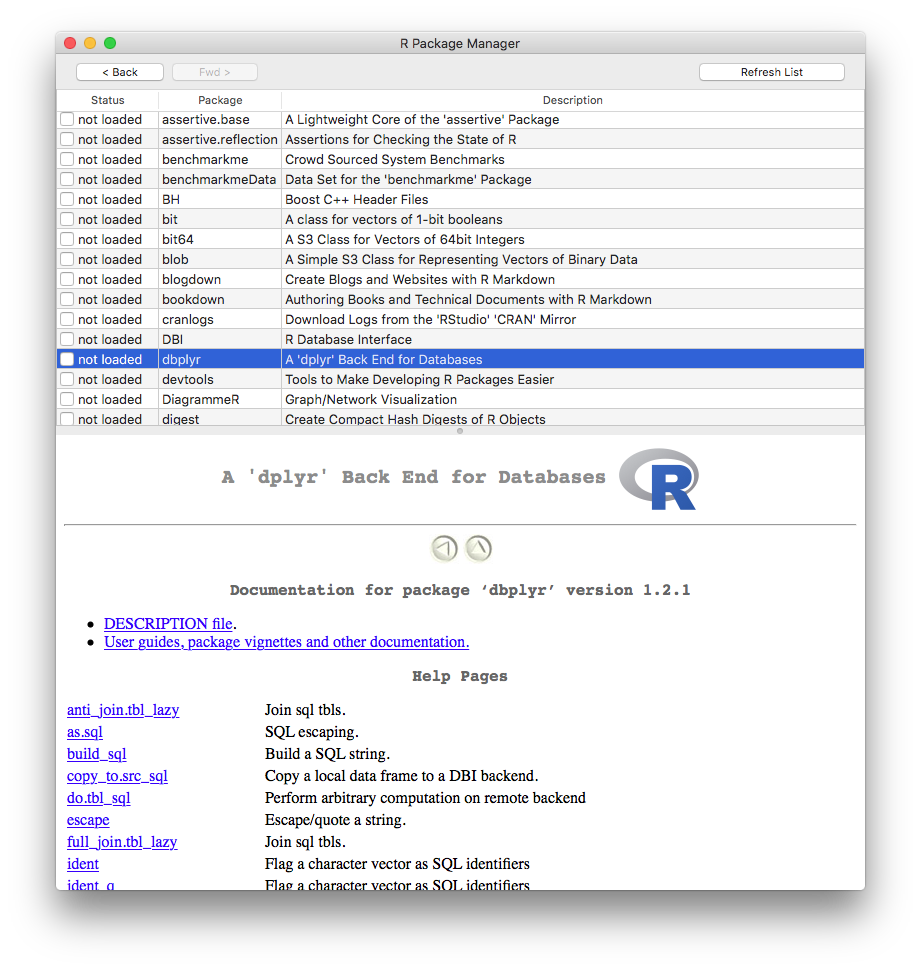
\includegraphics{images/R_Package_Manager.png}
\caption{\emph{\textbf{Above:} The Package Manager window lists
installed R packages and documentation.}}
\end{figure}

\hypertarget{r-packages}{%
\section{R Packages}\label{r-packages}}

\hypertarget{cran-package-repository}{%
\subsection{\texorpdfstring{\href{https://cran.r-project.org/}{CRAN
Package
Repository}}{CRAN Package Repository}}\label{cran-package-repository}}

\textbf{The Comprehensive R Archive Network} (CRAN) is a network of
\texttt{ftp} and Web servers around the world that store identical,
up-to-date versions of code and documentation for R. Using the nearest
\href{https://cran.r-project.org/}{CRAN Mirror} minimises network load.

\textbf{Official releases of R source code} (Unix and Windows) are
available on CRAN. The 2018-03-15 release is
\href{https://cran.r-project.org/src/base/R-3/R-3.4.4.tar.gz}{R-3.4.4
\emph{Someone to Lean On}}. Older releases are
\href{https://cran.r-project.org/src/base/}{available}.

\textbf{R documentation is available on CRAN} in
\href{https://cran.r-project.org/manuals.html\#R-admin}{HTML, PDF, and
EPUB} formats. These were created on \href{https://debian.org}{Debian
Linux} and may differ for Mac or Windows, but most parts will be
identical. The applicable manual is included in the R installation for
each OS.

\textbf{CRAN maintains tables of
\href{https://cran.r-project.org/}{available R packages}} sorted by
\href{https://cran.r-project.org/web/packages/available_packages_by_date.html}{date
of publication} and
\href{https://cran.r-project.org/web/packages/available_packages_by_name.html}{name}.
To assist \href{https://cran.r-project.org/}{searching for appropriate
packages}, CRAN offers discipline-based
\href{https://cran.r-project.org/web/views/}{Task Views}. On April 6
2018, the CRAN package repository contained 12,411 packages.

\textbf{All submitted packages are tested regularly} on Debian
GNU/Linux, Fedora, OS X, Solaris and Windows. The results are summarized
in the
\href{https://cran.r-project.org/web/checks/check_summary.html}{check
summary}.

\hypertarget{installing-cran-r-packages}{%
\subsection{Installing CRAN R
Packages}\label{installing-cran-r-packages}}

The R command \texttt{help("INSTALL")} or
\texttt{help("install.packages")} displays information on how to install
packages from CRAN. The general package installation command is:

\textbf{To download and install a package} --
\texttt{install.packages("PackageName")}\\
\textbf{To make its library available} -- \texttt{library(PackageName)}

\hypertarget{installing-packages-from-github}{%
\subsection{Installing Packages From
GitHub}\label{installing-packages-from-github}}

However, not all packages are available on CRAN, but must be downloaded
from \href{https://github.com/}{GitHub}. To enable this the
\texttt{devtools} package must be downloaded and made available:

\begin{quote}
\texttt{install.packages("devtools")}~\\
\texttt{library(devtools)}
\end{quote}

\begin{itemize}
\item
  \textbf{devtools'
  \texttt{install\_github("DeveloperName/PackageName")}} installs R
  packages from GitHub, but it requires the developers
  \href{https://help.github.com/articles/setting-your-username-in-git/}{GitHub
  name}.
\item
  \textbf{githubinstall's \texttt{githubinstall("PackageName")}} does
  not require the developers GitHub name. It also provides some helpful
  information on gitHub-hosted R packages hosted. This package can be
  installed from CRAN.
\end{itemize}

\textbf{If a repository package requires compiling the appropriate
compilers}, usually for \emph{C++} or \emph{FORTRAN}, \textbf{must be
already installed on your system}.

\textbf{A more detailed discussion for installing from GitHub} is
\href{https://cran.r-project.org/web/packages/githubinstall/vignettes/githubinstall.html}{available
here}.

\hypertarget{the-tidyverse}{%
\subsection{\texorpdfstring{\href{https://www.tidyverse.org/}{The
tidyverse}}{The tidyverse}}\label{the-tidyverse}}

\textbf{The \href{https://www.tidyverse.org/}{tidyverse} is a collection
of R packages designed to clean up datasets for analysis}. The
\emph{tidyverse philosophy} has become an important tool of Data
Science. \href{https://www.tidyverse.org/}{tidyverse} packages share the
same design philosophy, grammar, and structure. Ease of adoption and use
are fundamental principles for all packages of the
\href{https://www.tidyverse.org/}{tidyverse}.

\textbf{Core \texttt{tidyverse} packages:}

\begin{itemize}
\tightlist
\item
  \href{http://ggplot2.tidyverse.org/}{ggplot2} for data visualisation
\item
  \href{http://dplyr.tidyverse.org/}{dplyr} for data manipulation
\item
  \href{http://tidyr.tidyverse.org/}{tidyr} for data tidying
\item
  \href{http://readr.tidyverse.org/}{readr} for data import
\item
  \href{http://purrr.tidyverse.org/}{purrr} for functional programming
\item
  \href{http://tibble.tidyverse.org/}{tibble} for tibbles, a modern
  re-imagining of data frames
\end{itemize}

\textbf{Two other packages} are considered part of
\texttt{tidyverse\ core}:

\begin{itemize}
\tightlist
\item
  \href{http://stringr.tidyverse.org/}{stringr} for working with strings
\item
  \href{http://forcats.tidyverse.org/}{forecats} for resolving factors
\end{itemize}

\textbf{tidyverse packages sometimes conflict with other packages}.
You'll see this displayed on installing a
\href{https://www.tidyverse.org/}{tidyverse} package. You can:

\begin{itemize}
\item
  \textbf{list conflicts with other installed R packages at any time}\\
  with \texttt{tidyverse\_conflicts()}, and
\item
  \textbf{Check that all \href{https://www.tidyverse.org/}{tidyverse}
  packages are up-to-date}\\
  with \texttt{tidyverse\_update()}.
\end{itemize}

\textbf{\href{http://r4ds.had.co.nz/tidy-data.html}{Chapter 12} of the
seminal book \href{http://r4ds.had.co.nz/}{R For Data Science}} explains
in detail how to use \href{https://www.tidyverse.org/}{tidyverse}
packages to clean up data prior to analysis. Learning how to use the
\href{http://tidyverse.org/}{tidyverse} is the recommended first step to
mastering R programming for Data Science.

\hypertarget{ggplot2}{%
\subsubsection{\texorpdfstring{
\href{http://ggplot2.tidyverse.org/}{ggplot2}}{ ggplot2}}\label{ggplot2}}

\textbf{A system for declaratively creating graphics} based on
\href{vita.had.co.nz/papers/layered-grammar.pdf}{The Grammar of
Graphics}, \texttt{ggplot2} was created by
\href{http://hadley.nz/}{Hadley Wickham}. You provide the data; tell
\texttt{ggplot2} how to map variables to aesthetics and what graphical
primitives to use; it takes care of the details.

\hypertarget{dplyr}{%
\subsubsection{\texorpdfstring{
\href{http://dplyr.tidyverse.org/}{dplyr}}{ dplyr}}\label{dplyr}}

\textbf{A grammar of data manipulation}, \texttt{deplyr} provides a
consistent set of verbs to solve most common data manipulation
challenges. It abstracts how the data is stored, so it works as well
with remote databases as with local data frames, using exactly the same
R code.

\hypertarget{tidyr}{%
\subsubsection{\texorpdfstring{
\href{http://tidyr.tidyverse.org/}{tidyr}}{ tidyr}}\label{tidyr}}

\textbf{The goal of tidyr is to create tidy data}. Tidy data describes a
standard way of storing data so it can be used anywhere in the
\href{https://www.tidyverse.org/}{tidyverse}. If you ensure that your
data is tidy, youll spend less timing fighting with the tools and more
time working on analysis.

\hypertarget{readr}{%
\subsubsection{\texorpdfstring{
\href{http://readr.tidyverse.org/}{readr}}{ readr}}\label{readr}}

\textbf{Provides a fast and friendly way to read rectangular data} ---
comma-separated, tab-separated, fixed-width, and general-delimited
files, as well as tables separated by white space, and web log files.
\href{http://readr.tidyverse.org/}{readr} flexibly parses data while
failing cleanly if the data changes.

\hypertarget{purrr}{%
\subsubsection{\texorpdfstring{
\href{http://purrr.tidyverse.org/}{purrr}}{ purrr}}\label{purrr}}

\textbf{A complete toolset for working with functions and vectors},
\texttt{purrr} functions offer many advantages over the equivalents in
base R. For example, the \texttt{purrr} family of \texttt{map()}
functions replace many \texttt{for} loops with code that is both more
succinct and easier to read.

\hypertarget{tibble}{%
\subsubsection{\texorpdfstring{
\href{http://tibble.tidyverse.org/}{tibble}}{ tibble}}\label{tibble}}

\textbf{A modern reimagining of the data.frame}, \emph{tibbles} keep
what has proven to be effective. \emph{tibbles} are both lazy and surly:
they do less (they dont change variable names or types, or do partial
matching), and they complain more (for example when a variable does not
exist).

\hypertarget{stringr}{%
\subsubsection{\texorpdfstring{
\href{http://stringr.tidyverse.org/}{stringr}}{ stringr}}\label{stringr}}

\textbf{Designed to make working with strings as easy as possible}.
\href{http://stringr.tidyverse.org/}{stringr} focusses on the most
important and commonly-used string manipulation functions. It is built
on top of \href{https://github.com/gagolews/stringi}{stringi}, which
provides a comprehensive set covering almost anything you can imagine.

\hypertarget{forcats}{%
\subsubsection{\texorpdfstring{
\href{http://forcats.tidyverse.org/}{forcats}}{ forcats}}\label{forcats}}

\textbf{A suite of tools to solve problems with factors}. R uses factors
to handle categorical variables that have a fixed and known set of
possible values. Many base R functions convert character vectors to
factors, but \href{http://tidyverse.org/}{tidyverse} packages don't
create them automatically.

\hypertarget{rstudio-ide}{%
\chapter{RStudio IDE}\label{rstudio-ide}}

\href{https://www.rstudio.com/products/rstudio}{} \textbf{is a free,
open-source, professionally-designed IDE for programming in R} (and
other languages including Python and associated Python packages).

\href{https://en.wikipedia.org/wiki/RStudio}{RStudio} is available in
two free versions:

\begin{itemize}
\tightlist
\item
  \href{https://www.rstudio.com/products/rstudio/\#Desktop}{RStudio
  Desktop}, run locally as a desktop application. and
\item
  \href{https://www.rstudio.com/products/rstudio/\#Server}{RStudio
  Server}, which runs on a networked or remote Linux server.
\end{itemize}

\href{https://www.rstudio.com/products/rstudio-server-pro/}{RStudio
Server Pro} is a full-service, paid edition for business and government
use.

\textbf{The advantages of using RStudio include}:

\begin{itemize}
\tightlist
\item
  Free and open source for non-commercial use
\item
  Easy to install on Windows, Mac, and Linux
\item
  Well-designed, multi-pane GUI interface
\item
  Paid, full-service, professional versions
\item
  Git and Subversion versioning support
\item
  Can import data from online sources
\item
  Outputs to HTML, PDF, Word files
\item
  Built-in R package management
\item
  Keyboard shortcuts display
\item
  Active community support
\item
  Tab key code completion
\item
  Ongoing development
\item
  Well-documented
\item
  Code folding
\item
  It's So Cool
\item
  So is R!
\end{itemize}

From the
\href{https://www.rstudio.com/products/rstudio/features/}{RStudio web
Site}:

\textbf{An IDE that was built just for R}

\begin{itemize}
\tightlist
\item
  Syntax highlighting, code completion, and smart indentation
\item
  Execute R code directly from the source editor
\item
  Quickly jump to function definitions
\end{itemize}

\textbf{Bring your workflow together}

\begin{itemize}
\tightlist
\item
  Integrated R help and documentation
\item
  Easily manage multiple working directories using projects
\item
  Workspace browser and data viewer
\end{itemize}

\textbf{Powerful authoring \& Debugging}

\begin{itemize}
\tightlist
\item
  Interactive debugger to diagnose and fix errors quickly
\item
  Extensive package development tools
\item
  Authoring with Sweave and R Markdown
\end{itemize}

\hypertarget{the-rstudio-interface}{%
\section{The RStudio Interface}\label{the-rstudio-interface}}

\begin{figure}
\centering
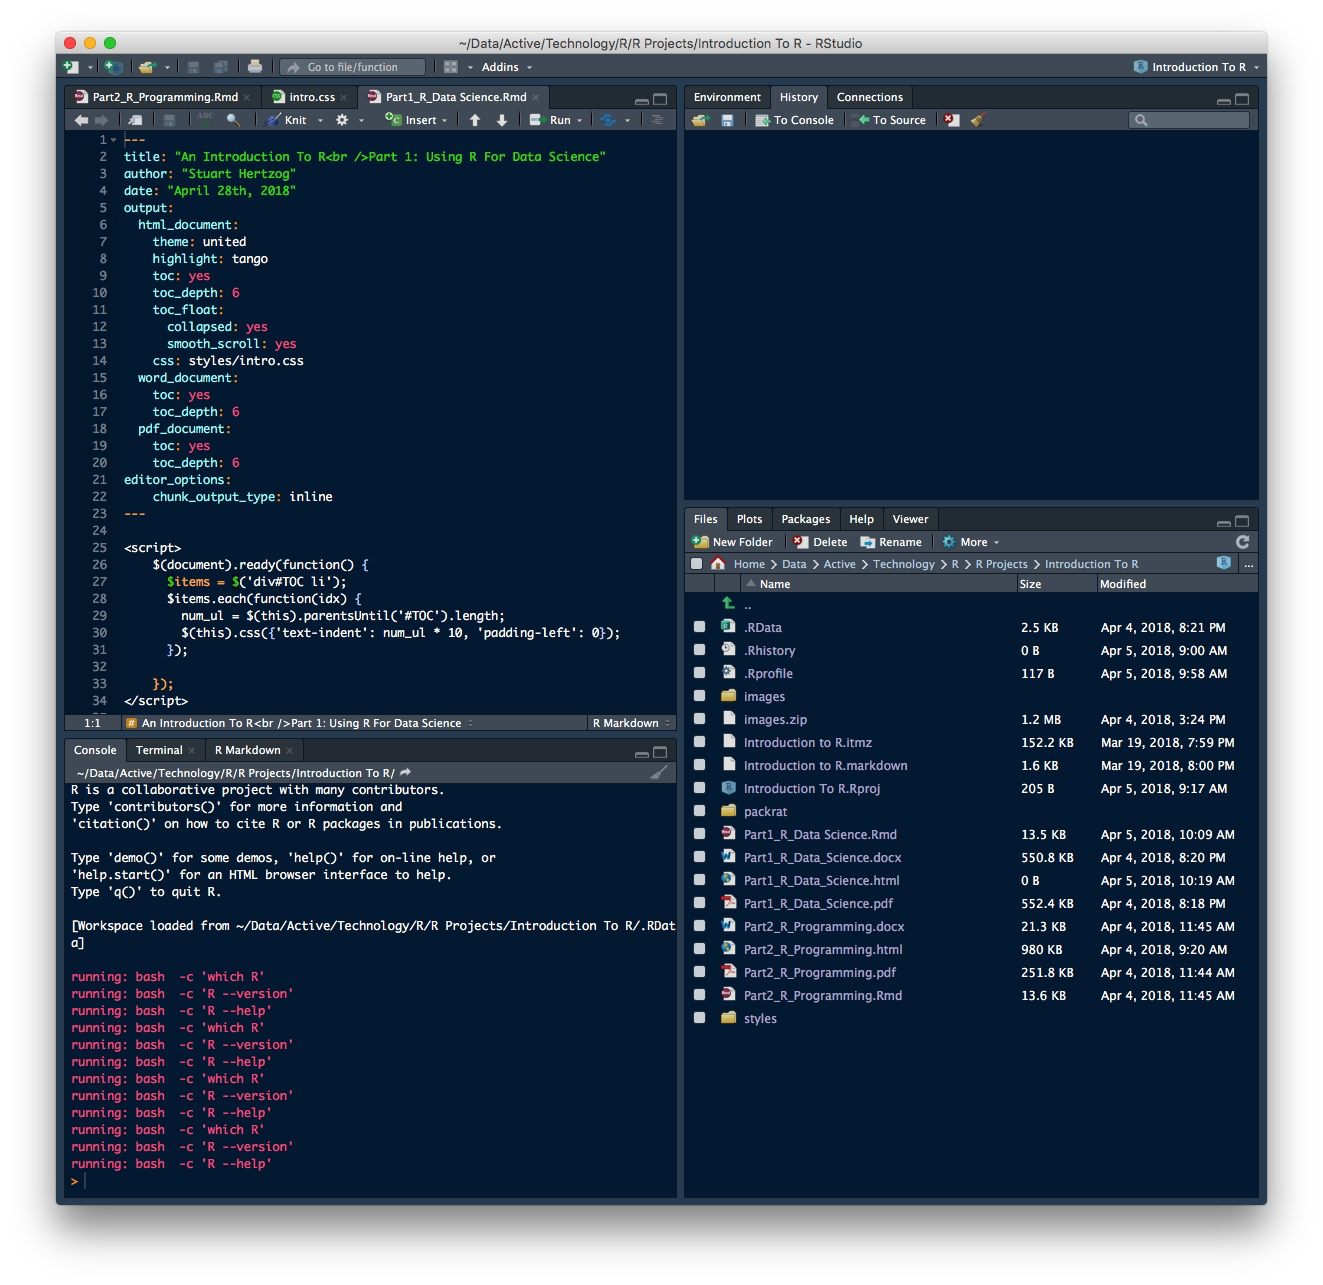
\includegraphics{images/RStudio_console.png}
\caption{\emph{\textbf{Above:} The four-pane default RStudio Console.
Pane arrangement can be changed.}}
\end{figure}

\textbf{The RStudio Console interface is flexible, rich, and capable}:

\begin{itemize}
\tightlist
\item
  Tabs in each pane display different aspects of the current project
\item
  Panes can share a column or be raised to fill an entire column
\item
  File and Viewer panes can be zoomed into a larger new window
\item
  Toolbars in each tab allow direct control of content elements
\item
  Console comands are integrated into the running OS and files
\item
  Console display can be changed by selecting a different theme
\item
  Code syntax colors can be changed with another editor theme
\end{itemize}

\hypertarget{rstudio-projects}{%
\section{RStudio Projects}\label{rstudio-projects}}

RStudio advises that \textbf{all data files and packages} belonging to a
project be contained in a dedicated directory as an \textbf{RStudio
Project} with an executable \textbf{\texttt{.Rproj} file}.

\textbf{Project management is built into RStudio}. Start a new Project
either from the \emph{File -\textgreater{} New Project} main menu, or
from the drop-down \textbf{Project menu} at the top right of the RStudio
window (left).

\emph{New Project\ldots{}} opens a dialogue window that enables a
Project to be created in a \emph{New} or \emph{Existing} directory, or
from a \emph{Version Control Repository}.

If an existing Project has unsaved changes, you will be asked to save
them.

\emph{Open Project\ldots{}} brings up a File dialogue to locate an
existing project directory and double-click its \texttt{.Rproj} file.

\emph{Open Project in New Session\ldots{}} allows you to create a new
Project in a new R session without closing the existing Project R
session.

\emph{Close Project} will close the running R session and after saving
any changes.

\textbf{Existing RStudio Projects} are listed below these to facilitate
switching between active projects. Entries are created when a project is
started by RStudio. This list can be emptied by selecting \emph{Clear
Project List}.

\textbf{Project Options} lets you set options specific only to the
running Project.

\hypertarget{package-management-in-rstudio}{%
\section{Package Management In
RStudio}\label{package-management-in-rstudio}}

\textbf{Package management is an integral part of the RStudio
interface}. The \emph{Packages} tab in the Files/Viewer pane shows all
locally-installed and system packages.

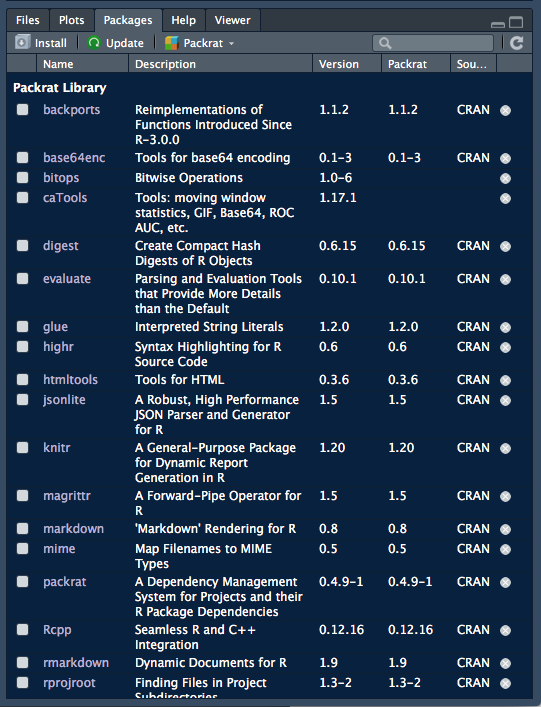
\includegraphics{images/RStudio_packages.png}

\textbf{Clicking the checkbox to the left of each package listing} will
load a package's library into memory and make its functions available.
The corresponding installation command will appear immediately in the
Console plus any warning messages.

\textbf{Packages with checkmarks have already been loaded}. Unclicking a
loaded package will unload it unless it is required by RMarkdown, in
which case a warning message will inform you of that restriction and the
package will remain loaded.

\textbf{There are two ways of installing packages} in the RStudio
interface:

\begin{itemize}
\tightlist
\item
  Using the \textbf{\emph{Install Packages} GUI}
\item
  Entering commands in the \textbf{Console}.
\end{itemize}

The progress of any compilation or installation will be displayed in the
Console.

\hypertarget{the-install-packages-gui}{%
\subsection{The Install Packages GUI}\label{the-install-packages-gui}}

\textbf{Clicking \emph{Install} on the Packages tab toolbar} opens an
\emph{Install Packages} dialogue (left) that gives the choice of
installing a package directly from CRAN or from a local package archive.

\textbf{Multiple packages can be installed} by separating the package
names with commas. This installs and makes the packages available for
use.

\textbf{The \emph{Install to Library} drop-down menu} allows you to
chose the Library where you want the package installed. The
\emph{default location} is selected: this is usually acceptable.

\textbf{The location of the R installation on your system} can be found
by entering \texttt{R.home(component\ =\ "home")} in the Console. Other
component values for the paths to specific directories of the current R
installation are \texttt{"bin"}, \texttt{"doc"}, \texttt{"etc"},
\texttt{"include"}, \texttt{library}, \texttt{"modules"} and
\texttt{"share"}.

\textbf{Clicking the \emph{Install dependencies} checkbox} will also
download and install any other packages required for the requested
package(s). This is recommended.

\textbf{NOTE: This option will not work when installing from a local
archive}. In this case the dependencies must be installed first, or the
installation will fail.

\#\#\#Installing From The Console

\textbf{Packages can be installed and loaded from the Console}. The
command sequence is:

\texttt{install.packages("PackageName")}\\
\texttt{library(PackageName)}

The delimiters \texttt{"\ "} or
\texttt{\textquotesingle{}\ \textquotesingle{}} must be used to install
a package.

Most R packages are hosted on CRAN, but some are only available on
\href{https://github.com}{GitHub} or
\href{https://bitbucket.org}{Bitbucket}. To install from these
locations, the \texttt{devtools} package first must be installed, as
\protect\hyperlink{installing-packages-from-github}{described above}.

\hypertarget{project-package-management}{%
\subsection{Project Package
Management}\label{project-package-management}}

\textbf{RStudio projects are built with different versions of
\texttt{R}} using the then-current versions of any installed packages.
As both \texttt{R} and \texttt{R\ packages} are constantly being
updated, this can cause problems when developing packages or
\texttt{RMarkdown} documents.

\textbf{There are four solutions to project package management}:

\begin{itemize}
\item
  Installing the
  \href{https://rstudio.github.io/packrat/}{\texttt{packrat}} package to
  write package versions in a \texttt{packrat.lock} text file and store
  the packages in a project \texttt{packrat} directory;
\item
  Using \href{https://mran.microsoft.com/timemachine}{MRAN} (Microsoft R
  Application Network) to determine dependencies based on the
  ``snapshot'' of CRAN that Microsoft has stored on a given day;
\item
  Installing the
  \href{https://cran.r-project.org/web/packages/checkpoint/vignettes/checkpoint.html}{\texttt{checkpoint}}
  package to choose package versions based on a given day in MRAN
  history.
\end{itemize}

For more information, see
\href{https://rviews.rstudio.com/2018/01/18/package-management-for-reproducible-r-code/}{Package
Management for Reproducible R Code}

\hypertarget{installing-and-using-packrat}{%
\subsection{\texorpdfstring{Installing And Using
\texttt{packrat}}{Installing And Using packrat}}\label{installing-and-using-packrat}}

\textbf{Packrat stores all added packages in its own directory library},
rather than relying on the user R library that is shared across all R
sessions.

The advantages of this are:

\begin{itemize}
\item
  \textbf{Isolation}: Installing a new or updated package for one
  project does not break other projects, and vice versa;
\item
  \textbf{Portability}: Enables moving projects from one computer to
  another, even across different platforms. (NOTE: this requires
  installation for each OS as the compiled libraries are not always
  identical);
\item
  \textbf{Reproducibility}: Ensures the correct package versions are
  assembled where and whenever the project is installed.
\end{itemize}

\textbf{\texttt{packrat} is integrated into the RStudio environment} so
it is easy to install and initiate. The \emph{Packages} tab in the
\emph{Files/Viewer} window has a \texttt{packrat} item menu. Clicking on
this brings up the \textbf{Packrat Options} window:

 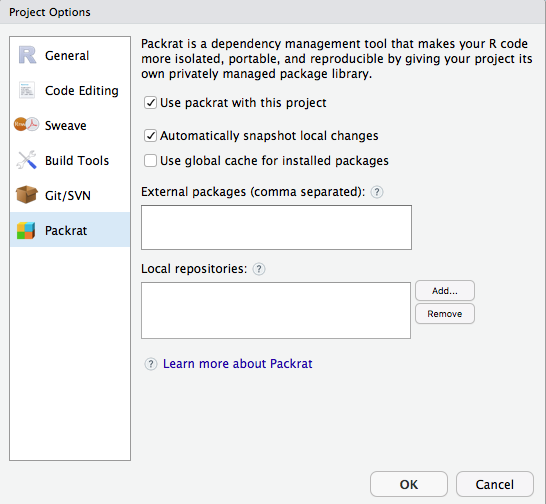
\includegraphics{images/RStudio_packrat_options.png}

\textbf{It's advisable to select the \emph{Automatically snapshot local
changes} option.}

\textbf{Clicking \texttt{OK} will download, install, and
initiate\texttt{packrat}} in exactly the same way the same as issuing
the commands from the Console:

\begin{quote}
install.packages(``packrat'')\\
packrat::init()
\end{quote}

\textbf{There also is an option in the \emph{New Project} window} to
create a new project with \texttt{packrat} pre-installed and initiated.

\textbf{Once \texttt{packrat} is up and running} the \emph{Packrat} link
will become a drop-down menu (left), containing the following options:

\emph{Check Library Status\ldots{}} -- shows if any packages require
updating

\emph{Clean Unused Packages} -- removes unneccessary packages. If you
want to keep a package from appearing in the Unused list, just add a
\texttt{library(PackageName)} call to any .R file in your Project
directory.

\emph{Export Project Bundle} -- creates a zipped bundle of your Project
in the \texttt{packrat} directory, for transport to another system. The
bundle contains application code, a manifest file, an html file, and a
\texttt{packrat} folder with a \texttt{packrat.lock} file.

\emph{Packrat Options\ldots{}} -- brings up the options window.
(\protect\hyperlink{packrat_options}{See above})

\textbf{For more information see}

\begin{itemize}
\tightlist
\item
  \href{https://rstudio.github.io/packrat/}{Packrat}
\item
  \href{https://rstudio.github.io/packrat/commands.html}{Packrat
  Commands}
\item
  \href{https://rstudio.github.io/packrat/walkthrough.html}{Packrat by
  example}
\item
  \href{https://rstudio.github.io/packrat/rstudio.html}{Using Packrat
  with RStudio}
\item
  \href{https://support.rstudio.com/hc/en-us/articles/115003639788-Bundle-Downloads}{Bundle
  Downloads}
\end{itemize}

\hypertarget{using-python-in-rstudio}{%
\section{Using Python In RStudio}\label{using-python-in-rstudio}}

\hypertarget{reticulate}{%
\subsection{\texorpdfstring{
\href{https://rstudio.github.io/reticulate/index.html}{reticulate}}{ reticulate}}\label{reticulate}}

Until recently it has not been possible to easily use Python in RStudio.
The newly-developed
\href{https://rstudio.github.io/reticulate/index.html}{reticulate}
package provides a \textbf{comprehensive set of tools for
interoperability between Python and R} within RStudio.

\textbf{\href{https://rstudio.github.io/reticulate/index.html}{reticulate}
includes facilities for}:

\begin{itemize}
\item
  \textbf{Calling Python from R} in a variety of ways including R
  Markdown, sourcing Python scripts, importing Python modules, and using
  Python interactively within an R session.
\item
  \textbf{Translation between R and Python objects} (for example,
  between R and Pandas data frames, or between R matrices and NumPy
  arrays).
\item
  \textbf{Flexible binding to different versions of Python} including
  virtual environments and Conda environments.
\end{itemize}

\textbf{\href{https://rstudio.github.io/reticulate/index.html}{reticulate}
embeds a Python session within your R session}, enabling seamless,
high-performance interoperability. If you are a Python developer, or an
R developer who uses Python for some of your work, or a member of data
science team that uses both languages,
\href{https://rstudio.github.io/reticulate/index.html}{reticulate} can
dramatically streamline your workflow.

\hypertarget{the-rstudio-ecosystem}{%
\chapter{The RStudio Ecosystem}\label{the-rstudio-ecosystem}}


\includegraphics{images/RStudio_full_logo.png}

\textbf{The RStudio IDE is the flagship of a comprehensive RStudio
ecosystem.}

\hypertarget{r-notebooks}{%
\section{R Notebooks}\label{r-notebooks}}

\href{https://rmarkdown.rstudio.com/r_notebooks.html}{R Notebooks} are
the most basic type of \protect\hyperlink{rmarkdown}{RMarkdown}
document. They are the RStudio equivalent to
\href{https://jupyter.org/}{Jupyter Notebooks}. As described by
\href{https://rmarkdown.rstudio.com/r_notebooks.html}{RStudio}:

\begin{quote}
An R Notebook is an R Markdown document with chunks that can be executed
independently and interactively, with output visible immediately beneath
the input.
\end{quote}

\textbf{Any R Markdown document can be used as a Notebook, and all R
Notebooks can be rendered to other R Markdown document types}.

\hypertarget{creating-an-r-notebook-file}{%
\subsection{Creating An R Notebook
File}\label{creating-an-r-notebook-file}}

\textbf{The RStudio menu item \emph{File -\textgreater{} New File
-\textgreater{} R Notebook}} creates a new
\href{https://rmarkdown.rstudio.com/r_notebooks.html}{RStudio Notebook}
containing instructions on how to use an R Notebook.

\begin{verbatim}
---
title: "R Notebook"
output:
  html_notebook
---

This is an [R Markdown](http://rmarkdown.rstudio.com) Notebook. When you execute code within the notebook, the results appear beneath the code. 

Try executing this chunk by clicking the *Run* button within the chunk or by placing your cursor inside it and pressing *Cmd+Shift+Enter*. 

```
{r}
plot(cars)
```

Add a new chunk by clicking the *Insert Chunk* button on the toolbar or by pressing *Cmd+Option+I*.

When you save the notebook, an HTML file containing the code and output will be saved alongside it (click the *Preview* button or press *Cmd+Shift+K* to preview the HTML file). 

The preview shows you a rendered HTML copy of the contents of the editor. Consequently, unlike *Knit*, *Preview* does not run any R code chunks. Instead, the output of the chunk when it was last run in the editor is displayed.
\end{verbatim}

For more information see
\href{https://rmarkdown.rstudio.com/r_notebooks.html}{RStudio Notebook}.

\hypertarget{r-notebook-html-files}{%
\subsection{R Notebook HTML files}\label{r-notebook-html-files}}

\textbf{An \href{https://rmarkdown.rstudio.com/r_notebook_format.html}{R
Notebook HTML file} is a special type of
\protect\hyperlink{r-notebook}{R Notebook}}.

It is an HTML file that uses the \texttt{.nb.html} extension and it
enables:

\begin{itemize}
\tightlist
\item
  \textbf{the source .Rmd document} and
\item
  \textbf{chunk outputs} to be recovered.
\end{itemize}

The \texttt{html\_notebook} output format is specified in the YAML
metadata:

\begin{verbatim}
title: "my_document_title"
output:
    html_notebook
\end{verbatim}

With the \texttt{\_yaml} file written this way, the command
\texttt{rmarkdown::render()} will create an \texttt{.nb.html} R Notebook
HTML Format file.

For more information, see
\href{https://rmarkdown.rstudio.com/r_notebook_format.html}{Details of
the R Notebook HTML Format}.

\textbf{Note}: The
\href{https://rmarkdown.rstudio.com/r_notebook_format.html\#generating-r-notebooks-with-custom-output}{RStudio
instructions} show an incorrect \texttt{YAML} header. You must use the
\texttt{\_yaml} format shown above or RStudio will throw an error and
not compile.

\hypertarget{rmarkdown}{%
\section{RMarkdown}\label{rmarkdown}}

\begin{quote}
R Markdown documents are fully reproducible. They use a productive
notebook interface to weave together narrative text and code to produce
elegantly-formatted output from multiple languages including R, Python,
and SQL.--- \href{https://rmarkdown.rstudio.com/}{\emph{RStudio
RMarkdown}}
\end{quote}

\textbf{\href{https://rmarkdown.rstudio.com/}{RMarkdown documents} are
the default RStudio document}. They are plain-text files with the
\texttt{.Rmd} extension and can be used to generate many different types
of output. The main ones are:

\begin{itemize}
\tightlist
\item
  \href{https://rmarkdown.rstudio.com/html_document_format.html}{HTML
  documents} -- \texttt{.html}
\item
  \href{https://rmarkdown.rstudio.com/pdf_document_format.html}{PDF
  Documents} -- \texttt{.pdf}
\item
  \href{https://rmarkdown.rstudio.com/word_document_format.html}{Word
  Documents} -- \texttt{.docx}
\end{itemize}

In addition to the standard output formats (above), RMarkdown documents
can generate output in many other formats, via the
\protect\hyperlink{pandoc}{pandoc} conversion engine.

\href{https://rmarkdown.rstudio.com/beamer_presentation_format.html}{Beamer},
\href{https://rmarkdown.rstudio.com/ioslides_presentation_format.html}{HTML5
slides},
\href{https://rmarkdown.rstudio.com/tufte_handout_format.html}{Tufte-style
handouts}, \href{https://bookdown.org/yihui/bookdown/}{books},
\href{https://rmarkdown.rstudio.com/flexdashboard/}{dashboards},
\href{https://rmarkdown.rstudio.com/authoring_shiny.html}{interactive
documents}, \href{https://github.com/rstudio/rticles}{scientific
articles}, and
\href{https://rmarkdown.rstudio.com/rmarkdown_websites.html}{websites}.

\href{https://rmarkdown.rstudio.com/gallery.html}{\textbf{RStudio
maintains a gallery of examples}} of the many uses of RMarkdown.

\hypertarget{knitr}{%
\subsection{knitr}\label{knitr}}

\begin{quote}
RMarkdown uses the \href{https://yihui.name/knitr/}{knitr} report
generation package to output to the different file formats.
\end{quote}

\textbf{The \texttt{knitr} package enables integration of R code into
\href{https://en.wikipedia.org/wiki/LaTeX}{LaTeX},
\href{https://en.wikipedia.org/wiki/LyX}{LyX},
\href{https://en.wikipedia.org/wiki/HTML}{HTML},
\href{https://en.wikipedia.org/wiki/Markdown}{Markdown},
\href{https://en.wikipedia.org/wiki/AsciiDoc}{AsciiDoc}, and
\href{https://en.wikipedia.org/wiki/ReStructuredText}{reStructuredText}
documents}. It can execute code chunks in a variety of languages via
\href{https://rmarkdown.rstudio.com/authoring_knitr_engines.html}{knitr
Language Engines}, including for:

\begin{itemize}
\tightlist
\item
  R
\item
  Python
\item
  SQL
\item
  Bash
\item
  Rcpp
\item
  Stan
\item
  JavaScript
\item
  CSS
\end{itemize}

\textbf{To process a code chunk using an alternate language engine}
simply use the name of the engine in place of \texttt{\{r\}} in the
chunk declaration, for example:

\begin{verbatim}

```bash
cat flights1.csv flights2.csv flights3.csv > flights.csv
```
\end{verbatim}

\hypertarget{code-chunk-options}{%
\subsubsection{Code Chunk Options}\label{code-chunk-options}}

\textbf{RMarkdown code chunk processing can be controlled} by including
\href{https://rmarkdown.rstudio.com/lesson-3.html}{\emph{Chunk Options}}
in the \emph{Chunk Declaration}, for example:

\texttt{\{r,\ include\ =\ FALSE}\} prevents code and results from
appearing.\\
R Markdown still runs the code and the results can be used by other
chunks.\\
\texttt{\{r,\ eval\ =\ FALSE}\} prevents to code from running but it
still appears. \texttt{\{r,\ echo\ =\ FALSE}\} prevents code but not the
results from appearing.\\
This is a useful way to embed figures.\\
\texttt{\{r,\ message\ =\ FALSE}\} prevents messages generated by code
from appearing.\\
\texttt{\{r,\ warning\ =\ FALSE}\} prevents warnings generated by code
from appearing.\\
\texttt{\{r,\ fig.cap\ =\ "..."}\} adds a caption to graphical results.

The
\href{https://www.rstudio.com/wp-content/uploads/2015/03/rmarkdown-reference.pdf}{R
Markdown Reference Guide (.pdf)} has a list of useful options.
\href{https://yihui.name/knitr/options/}{Yihui's \texttt{knitr} options}
has full documentation of all \texttt{knitr} code processing controls.

\hypertarget{pandoc}{%
\subsection{pandoc}\label{pandoc}}

The RStudio installation includes \href{http://pandoc.org/}{pandoc},
which is used for conversion between RMarkdown and
\href{https://rmarkdown.rstudio.com/formats.html}{the various output
formats}. You may have to
\href{http://pandoc.org/installing.html}{install pandoc on your system}
for conversion to take place, especially for \texttt{.pdf} output, which
goes through an intermediate \texttt{LaTeX} stage.

\texttt{pandoc} can also be run from the commond line if it is installed
separately. This is explained in detail in the
\href{http://pandoc.org/MANUAL.html}{pandoc manual}.

\hypertarget{shiny}{%
\section{Shiny}\label{shiny}}

\begin{quote}
\href{http://shiny.rstudio.com/}{Shiny} is an R package that makes it
easy to build interactive web apps straight from R. You can host
standalone apps on a webpage or embed them in
\href{http://rmarkdown.rstudio.com/}{R Markdown} documents or build
\href{http://rstudio.github.io/shinydashboard/}{dashboards}. You can
also extend your Shiny apps with
\href{http://rstudio.github.io/shinythemes/}{CSS themes},
\href{http://www.htmlwidgets.org/}{htmlwidgets}, and JavaScript
\href{https://github.com/daattali/shinyjs/blob/master/README.md}{actions}.
--- \href{http://shiny.rstudio.com/}{\emph{RStudio Shiny}}
\end{quote}

\textbf{\href{http://shiny.rstudio.com/}{RStudio's Shiny} is a Web
application framework for R that takes static
\protect\hyperlink{rmarkdown}{RMarkdown documents} and
\href{https://rmarkdown.rstudio.com/html_document_format.html}{Web
sites} to the next level}.

There is no limit to building online documentation, interactive
tutorials, and statistical data interfaces with these powerful R
packages:

\begin{itemize}
\item
  \href{http://www.htmlwidgets.org/}{\texttt{htmlwidgets}} enables
  JavaScript visualisations and interactive components to be
  incorporated into \protect\hyperlink{rmarkdown}{R Markdown documents}
  and Shiny web applications, as shown in this
  \href{http://www.htmlwidgets.org/showcase_leaflet.html}{showcase} and
  this \href{http://www.htmlwidgets.org/}{gallery}
\item
  \href{http://rstudio.github.io/crosstalk/}{\texttt{crosstalk}} wires
  widgets together, including linked brushing between widgets and client
  side filtering
\item
  \href{http://rstudio.github.io/shinydashboard/}{\texttt{shinydashboard}}
  makes it easy to create all kinds of Web dashboards, as shown in
  \href{http://rstudio.github.io/shinydashboard/examples.html}{these
  examples}
\end{itemize}

and others:

\begin{itemize}
\tightlist
\item
  \href{https://github.com/psolymos/intrval}{\texttt{intrval}} can be
  used to build for example, a
  \href{http://peter.solymos.org/code/2018/03/08/shiny-slider-examples-with-the-intrval-r-package.html}{Web
  slider}
\end{itemize}

We will explore \href{http://shiny.rstudio.com/}{building Shiny apps} in
a future Tutorial.

\hypertarget{shiny-server}{%
\subsection{Shiny Server}\label{shiny-server}}

\href{https://www.rstudio.com/products/shiny/shiny-server/}{Shiny
Server} makes your \href{http://shiny.rstudio.com/}{Shiny Web apps}
accessible on a local network, an Enterprise server, or on the Internet.
There are two flavours of server:

\begin{itemize}
\tightlist
\item
  \href{https://www.rstudio.com/products/shiny/download-server/}{Shiny
  Server Open Source} and
\item
  \href{https://www.rstudio.com/products/rstudio-server-pro/}{Shiny
  Server Pro}
\end{itemize}

Documentation is available for:

\begin{itemize}
\tightlist
\item
  \href{https://www.rstudio.com/products/shiny/download-server/}{Installing
  Shiny Server Open Source}
\item
  \href{http://docs.rstudio.com/shiny-server/}{Shiny Server Pro Admin
  Guide}
\item
  \href{http://docs.rstudio.com/shinyapps.io/index.html}{shinyapps.io
  User Guide}
\end{itemize}

Shiny Apps can be available to an Intranet or to the Internet via:

\begin{itemize}
\tightlist
\item
  \href{https://www.rstudio.com/products/rstudio-server-pro/}{An
  Enterprise Server}
\item
  \href{https://www.rstudio.com/products/connect/}{RStudio Connect}
\item
  \href{https://www.rstudio.com/products/shinyapps/}{shinyapps.io}
\end{itemize}

The difference between the latter two is
\href{https://support.rstudio.com/hc/en-us/articles/217240558-What-is-the-difference-between-shinyapps-io-and-Shiny-Server-Pro-}{explained
here}.

\hypertarget{bookdown}{%
\section{bookdown}\label{bookdown}}

\begin{quote}
\href{https://github.com/rstudio/bookdown}{\texttt{bookdown}} is an
open-source R package that makes it really easy to creates online books
and technical documents using \protect\hyperlink{rmarkdown}{RMarkdown}.
\end{quote}

\textbf{\texttt{bookdown} books open a new avenue for Web-enabled book
publishing}.

They are essentially \textbf{responsive RMarkdown Web sites}, complete
with content navigation, plus the ability to display and process
computer code using a wide range of programming languages, including
interactive
\href{http://rstudio.github.io/shinydashboard/examples.html}{Shiny
dashboards} and \href{http://shiny.rstudio.com/gallery/}{Web apps}.

\textbf{\texttt{bookdown} has added a few important missing features}
related to writing books, such as figure and table caption numbering and
cross-references, and the ability to embed
\href{https://www.rstudio.com/products/shinyapps/}{HTML widgets} or
\href{http://shiny.rstudio.com/gallery/}{Shiny apps}.

\textbf{Developed and maintained by RStudio software engineer
\href{http://yihui.name}{Yihui Xie}}, \texttt{bookdown} books can be
published on \href{https://bookdown.org/}{bookdown.org}, a free service
provided by \href{https://www.rstudio.com/about/}{RStudio Inc}. Books
are available for download, and the author holds full copyright.

\href{https://bookdown.org/}{}

\textbf{Fully-documented} in --- of course! --- a
\href{https://bookdown.org/yihui/bookdown/}{\texttt{bookdown} book
called \emph{bookdown}}, the \texttt{bookdown} package uses many of the
same conventions as \protect\hyperlink{rmarkdown}{other RMarkdown
document types}, so conversion of any RStudio project to an online book
is relatively straightforward.

\href{https://github.com/rstudio/bookdown-demo}{A Minimal Book Example}
can be cloned from GitHub. It can also be downloaded as a
\href{https://github.com/rstudio/bookdown-demo/archive/master.zip}{\texttt{.zip}
file} if you are \href{http://rogerdudler.github.io/git-guide/}{not
familiar with GitHub}.

\hypertarget{bookdown-installation}{%
\subsection{\texorpdfstring{\texttt{bookdown}
Installation}{bookdown Installation}}\label{bookdown-installation}}

\href{https://bookdown.org/home/getting-started.html}{Installation}
requires the
\href{https://www.rstudio.com/products/rpackages/devtools/}{devtools} R
package to be first installed, after which \texttt{bookdown} can be
installed from \href{https://github.com/rstudio/bookdown}{its GitHub
repository}:

\begin{Shaded}
\begin{Highlighting}[]
\KeywordTok{install.packages}\NormalTok{(}\StringTok{"devtools"}\NormalTok{)}
\NormalTok{devtools}\OperatorTok{::}\KeywordTok{install_github}\NormalTok{(}\StringTok{"rstudio/bookdown"}\NormalTok{)}
\end{Highlighting}
\end{Shaded}

\hypertarget{tinytex}{%
\subsection{\texorpdfstring{\texttt{tinytex}}{tinytex}}\label{tinytex}}

\textbf{PDF output requires some version of the
\href{https://www.latex-project.org/}{LaTeX} typesetting system} to be
installed. LaTeX is not a stand-alone typesetting program in itself, but
document preparation software that runs on top of Donald E. Knuth's
\href{https://en.wikipedia.org/wiki/TeX}{TeX typesetting system}.

\textbf{\href{https://www.latex-project.org/get/\#tex-distributions}{TeX
distributions} usually bundle together all the parts needed} for a
working TeX system. \href{https://www.latex-project.org/}{LaTeX} and
many of the packages built on it form an important component of any
modern TeX distribution.

\textbf{As this is a large package consisting of many gigabytes of
files} that users may not wish to install,
\href{https://yihui.name/tinytex/}{Yihui Xie wrote \texttt{tinytex}}, a
lightweight, cross-platform, portable, and easy-to-maintain LaTeX
distribution based on \href{https://en.wikipedia.org/wiki/TeX_Live}{TeX
Live}.

\hypertarget{tinytex-installation}{%
\subsubsection{\texorpdfstring{\texttt{tinytex}
Installation}{tinytex Installation}}\label{tinytex-installation}}

Installation of \texttt{tinytex} is accomplished with:

\begin{Shaded}
\begin{Highlighting}[]
\KeywordTok{install.packages}\NormalTok{(}\KeywordTok{c}\NormalTok{(}\StringTok{'tinytex'}\NormalTok{, }\StringTok{'rmarkdown'}\NormalTok{))}
\NormalTok{tinytex}\OperatorTok{::}\KeywordTok{install_tinytex}\NormalTok{()}
\end{Highlighting}
\end{Shaded}

{}
\textbf{\href{https://rmarkdown.rstudio.com/pdf_document_format.html}{PDF
output} (including
\href{https://rmarkdown.rstudio.com/beamer_presentation_format.html}{Beamer
slides}) requires a full TeX installation.}

\hypertarget{blogdown}{%
\section{blogdown}\label{blogdown}}

\begin{quote}
Just as \href{https://wordpress.com/}{WordPress} changed the Web by
bringing blogging to the masses,
\href{https://bookdown.org/yihui/blogdown/}{blogdown} has opened a path
for the more computer-savvy to create quick-loading, static blog sites
using \protect\hyperlink{rmarkdown}{RMarkdown}.
\end{quote}

Not content with authoring
\protect\hyperlink{bookdown}{\texttt{bookdown}}, RStudio developer
\href{http://yihui.name}{Yihui Xie} took the next logical step by
writing the
\href{https://bookdown.org/yihui/blogdown/}{\texttt{blogdown} R
package}.

\textbf{Based on the \href{https://gohugo.io/}{Hugo website framework},
\texttt{blogdown} lets you write posts in RStudio as RMarkdown.Rmd files
These are automatically converted to blog posts for uploading to a
hosting service, including \href{https://pages.github.com/}{GitHub
pages}}.

\hypertarget{learning-blogdown}{%
\subsection{\texorpdfstring{Learning
\texttt{blogdown}}{Learning blogdown}}\label{learning-blogdown}}

It is advisable to first read Yihui Xie and Alison Presmanes Hill's
\texttt{bookdown} book
\href{https://bookdown.org/yihui/blogdown/}{Creating Websites with R
Markdown} to become familiar with \texttt{bookdown} concepts and the
\href{https://gohugo.io/}{Hugo framework} before you embark on creating
your first blog site.

\textbf{These links offer practical Setup hints and guidance:}

\hypertarget{blogdown-setup}{%
\subsubsection{blogdown Setup}\label{blogdown-setup}}

\begin{itemize}
\tightlist
\item
  \href{https://alison.rbind.io/post/up-and-running-with-blogdown/}{Up
  and running with blogdown \textbar{} Alison Presmanes Hill}
\item
  \href{https://www.znmeb.mobi/2017/05/12/getting-started-with-blogdown/}{Getting
  Started With Blogdown \textbar{} Borasky Research Journal}
\item
  \href{https://aurora-mareviv.github.io/talesofr/2018/02/r-blogdown-setup-in-github-2/}{R
  Blogdown Setup in GitHub (2) \textbar{} Tales of R}
\item
  \href{https://support.rbind.io/2017/04/25/yihui-website/\#fnref:For-two-reasons}{A
  Technical Introduction to Yihui's personal website}
\item
  \href{https://support.rbind.io/2017/04/28/daijiang-website/\#fnref:frankly-I-cloned}{A
  not-so-technical introduction to Daijiang's personal website}
\end{itemize}

\hypertarget{blogdown-links}{%
\subsubsection{blogdown Links}\label{blogdown-links}}

\begin{itemize}
\tightlist
\item
  \href{https://bookdown.org/yihui/blogdown/}{blogdown: Creating
  Websites with R Markdown}
\item
  \href{https://blog.rstudio.com/2017/09/11/announcing-blogdown/}{Announcing
  blogdown - Yihui Xie, RStudio 2017-09-11}
\item
  \href{https://github.com/rstudio/blogdown}{GitHub - rstudio/blogdown:
  Create Blogs and Websites with R Markdown}
\item
  \href{https://github.com/rbind/blogdown-demo}{GitHub -
  rbind/blogdown-demo: A minimal website example using blogdown}
\item
  \href{https://twitter.com/hashtag/blogdown}{Twitter hashtag
  \#blogdown}
\end{itemize}

\hypertarget{hugo-themes}{%
\subsection{Hugo Themes}\label{hugo-themes}}

\textbf{\texttt{blogdown} uses \href{https://gohugo.io/themes/}{Hugo
themes} to style the look and feel of its blogs}. The default theme for
\texttt{blogdown} is
\href{https://github.com/yihui/hugo-lithium}{\emph{hugo-lithium}}, a
minimal theme that offers several options, detailed in
\href{https://bookdown.org/yihui/blogdown/themes.html\#the-default-theme}{Section
2.4.1} of the \texttt{blogdown} book. The base theme can be modified to
suit your taste, or it can be replaced by another theme.

\textbf{The \href{https://gohugo.io/}{Hugo web site} showcases many
\href{https://themes.gohugo.io}{user-contributed themes}}. These can be
examined online and downloaded for use as-is or as a starting point for
themeing.

\hypertarget{hugo-links}{%
\subsubsection{Hugo Links}\label{hugo-links}}

\begin{itemize}
\tightlist
\item
  \href{https://gohugo.io/}{Hugo} --- world's fastest (?) framework for
  building websites
\item
  \href{https://gohugo.io/getting-started/installing/}{Hugo Setup Guide}
  --- applies to \texttt{blogdown} blog sites
\item
  \href{https://gohugo.io/themes/}{Hugo Themeing} --- how to choose and
  fine-tune a blog
\item
  \href{https://themes.gohugo.io}{Contributed Hugo Themes} -- hundreds
  of excellent Hugo themes
\item
  \href{https://riinu.netlify.com/2018/02/converting-old-wordpress-posts-to-hugo/}{Converting
  Old Wordpress Posts To Hugo} --- goodbye WordPress!
\end{itemize}

\hypertarget{blogdown-blogs}{%
\subsection{\texorpdfstring{\texttt{blogdown}
Blogs}{blogdown Blogs}}\label{blogdown-blogs}}

A list of R-related \texttt{blogdown} blogs is kept at
\href{https://github.com/rbind}{rbind on Github}. R-blogs made with
\texttt{blogdown} can be viewed
\href{https://github.com/search?q=org\%3Arbind+blogdown}{here}.

An interesting and uncluttered example is
\href{https://simplystatistics.org/}{Simply Statistics}, a statistics
blog by Rafa Irizarry, Roger Peng, and Jeff Leek.

\hypertarget{rstudio-products}{%
\section{RStudio Products}\label{rstudio-products}}


\includegraphics{images/RStudio_full_logo.png}

\textbf{Some RStudio products are open-source and free for student and
personal use}. Others are priced for professional or Enterprise
deployment.

\hypertarget{software}{%
\subsection{Software}\label{software}}

\begin{itemize}
\tightlist
\item
  \href{https://rmarkdown.rstudio.com/r_notebooks.html}{R Notebooks} ---
  equivalent to \href{https://jupyter.org/}{Jupyter Notebooks}
\item
  \href{https://rmarkdown.rstudio.com/}{RMarkdown} --- creates
  \texttt{.Rmd} files using
  \href{https://rmarkdown.rstudio.com/authoring_pandoc_markdown.html}{Pandoc
  Markdown}
\item
  \href{https://www.rstudio.com/products/rpackages/}{R Packages} ---
  available on \href{https://cran.r-project.org/}{CRAN} and
  \href{https://github.com/rstudio}{GitHub}
\item
  \href{https://www.rstudio.com/products/rstudio/\#Desktop}{RStudio
  Desktop} --- the RStudio IDE, also on
  \href{https://github.com/rstudio}{GitHub}
\item
  \href{https://www.rstudio.com/products/rstudio/\#Server}{RStudio
  Server} --- free for personal and local Network use
\item
  \href{https://www.rstudio.com/products/shiny/}{Shiny} --- build
  interactive Web pages and
  \href{https://www.javascript.com}{JavaScript} apps
\item
  \href{https://www.rstudio.com/products/shiny/shiny-server2/}{Shiny
  Server} --- free for local network and Web access behind a firewall
\end{itemize}

\hypertarget{cloud-services}{%
\subsection{Cloud Services}\label{cloud-services}}

\begin{itemize}
\tightlist
\item
  \href{https://www.rstudio.com/products/rstudio-server-pro/}{RStudio
  Server Pro} -- enhanced admin, Enterprise security and pricing
\item
  \href{https://www.rstudio.com/products/connect/}{RStudio Connect} --
  team management, Enterprise security and pricing
\item
  \href{https://rstudio.cloud/}{RStudio Cloud (in alpha)} --- Do, Share,
  Teach, and Learn Data Science
\item
  \href{https://www.rstudio.com/products/shiny-server-pro/}{Shiny Server
  Pro} -- share Shiny apps, Enterprise security and pricing
\item
  \href{https://www.rstudio.com/products/shinyapps/}{shinyapps.io} --
  deploy Shiny apps, enhanced security, scalable
\item
  \href{https://bookdown.org/}{Bookdown Book Publishing} --- free for
  \texttt{bookdown} static page books
\end{itemize}

\hypertarget{resources}{%
\subsection{Resources}\label{resources}}

\begin{itemize}
\tightlist
\item
  \href{https://www.rstudio.com/resources/cheatsheets/}{RStudio Cheat
  Sheets} --- PDF format
\item
  \href{https://community.rstudio.com/}{RStudio Community} --- register
  for full Forum access
\item
  \href{https://support.rstudio.com/hc/en-us/categories/200035113-Documentation}{RStudio
  Documentation} --- Help articles for all RStudio products
\item
  \href{https://support.rstudio.com/hc/en-us/articles/234653607-Getting-Started-with-RStudio-Server}{RStudio
  Server\textgreater{} Getting Started} --- lists many links for setup
  and use
\item
  \href{http://docs.rstudio.com/ide/server-pro/}{RStudio Server Pro
  Admin. Guide} --- web-accessible User Manual
\end{itemize}

\hypertarget{the-fundamentals-of-r}{%
\chapter{The Fundamentals of R}\label{the-fundamentals-of-r}}

\hypertarget{four-fundamentals}{%
\section{Four Fundamentals}\label{four-fundamentals}}

The essence of R:

\begin{Shaded}
\begin{Highlighting}[]
\NormalTok{R <-}\StringTok{ }\KeywordTok{c}\NormalTok{(}\DecValTok{1}\OperatorTok{:}\DecValTok{4}\NormalTok{)}
\NormalTok{R}
\end{Highlighting}
\end{Shaded}

\begin{verbatim}
## [1] 1 2 3 4
\end{verbatim}

(See \protect\hyperlink{vectors}{Vectors} later).

\textbf{{[}One{]}} important difference about R:

\begin{itemize}
\tightlist
\item
  \textbf{Vector-based}: R is not a procedural language
\end{itemize}

\textbf{{[}Two{]}} reasons to use R for Data Science:

\begin{itemize}
\tightlist
\item
  \textbf{Designed for data}: R can manipulate big data sets
\item
  \textbf{Graphics Are Graspable}: people understand graphical data
\end{itemize}

\textbf{{[}Three{]}} fundamental principles of R per
\href{https://en.wikipedia.org/wiki/John_Chambers_(statistician)}{John
Chambers}:

\begin{itemize}
\tightlist
\item
  \textbf{Objects}: Everything that exists in R is an object
\item
  \textbf{Functions}: Everything that happens in R is a function call
\item
  \textbf{Interfaces}: to other softwares are an integral part of R
\end{itemize}

\textbf{{[}Four{]}} ways of programming R:

\begin{itemize}
\tightlist
\item
  \textbf{Command line}: entering R commands in a terminal
\item
  \textbf{Source file}: running a set of commands from a saved file
\item
  \textbf{R GUI interface}: available for Mac, WIndows, and Linux
\item
  \textbf{Code chunks in RStudio}: allows debugging as you write
\end{itemize}

\hypertarget{basic-maths}{%
\section{Basic Maths}\label{basic-maths}}

R has all the basic mathematical functions:

\begin{Shaded}
\begin{Highlighting}[]
\DecValTok{1} \OperatorTok{+}\StringTok{ }\DecValTok{1}
\end{Highlighting}
\end{Shaded}

\begin{verbatim}
## [1] 2
\end{verbatim}

\begin{Shaded}
\begin{Highlighting}[]
\DecValTok{1} \OperatorTok{+}\StringTok{ }\DecValTok{2} \OperatorTok{+}\StringTok{ }\DecValTok{3}
\end{Highlighting}
\end{Shaded}

\begin{verbatim}
## [1] 6
\end{verbatim}

\begin{Shaded}
\begin{Highlighting}[]
\DecValTok{3} \OperatorTok{*}\StringTok{ }\DecValTok{7} \OperatorTok{*}\StringTok{ }\DecValTok{2}
\end{Highlighting}
\end{Shaded}

\begin{verbatim}
## [1] 42
\end{verbatim}

\begin{Shaded}
\begin{Highlighting}[]
\DecValTok{4} \OperatorTok{/}\StringTok{ }\DecValTok{3}
\end{Highlighting}
\end{Shaded}

\begin{verbatim}
## [1] 1.333333
\end{verbatim}

R obeys the standard order of mathematical operations (\textbf{PEMDAS}):

\begin{enumerate}
\def\labelenumi{\arabic{enumi}.}
\tightlist
\item
  \textbf{P}arentheses ( )
\item
  \textbf{E}xponents \^{}
\item
  \textbf{M}ultiplication x
\item
  \textbf{D}ivision\\
\item
  \textbf{A}ddition +
\item
  \textbf{S}ubtraction -
\end{enumerate}

\begin{Shaded}
\begin{Highlighting}[]
\NormalTok{(}\DecValTok{2} \OperatorTok{^}\StringTok{ }\DecValTok{5}\NormalTok{) }\OperatorTok{+}\StringTok{ }\NormalTok{(}\DecValTok{2} \OperatorTok{*}\StringTok{ }\DecValTok{5}\NormalTok{)}
\end{Highlighting}
\end{Shaded}

\begin{verbatim}
## [1] 42
\end{verbatim}

The use of white space between operators is recommended.

\hypertarget{variables}{%
\section{Variables}\label{variables}}

Unlike statically-typed languages such a C++, R does not require
variable types to be declared. An R variable can represent any data type
or R object, such as a function, result, or graphical plot. R variables
can be redeclared.

\begin{itemize}
\tightlist
\item
  Variable names can \textbf{contain alphanumeric characters}

  \begin{itemize}
  \tightlist
  \item
    but not \textbf{periods \texttt{.} or underscores \texttt{\_}}
  \end{itemize}
\item
  \textbf{They cannot \emph{start} with a number or underscore}
\item
  Variable names are \textbf{case sensitive}
\end{itemize}

\hypertarget{assigning-variables}{%
\subsection{Assigning variables}\label{assigning-variables}}

R variable assignment operators are \texttt{\textless{}-} (default) and
\texttt{=} (acceptable).

\begin{Shaded}
\begin{Highlighting}[]
\NormalTok{x <-}\StringTok{ }\DecValTok{2}
\NormalTok{x}
\end{Highlighting}
\end{Shaded}

\begin{verbatim}
## [1] 2
\end{verbatim}

\begin{Shaded}
\begin{Highlighting}[]
\NormalTok{y =}\StringTok{ }\DecValTok{5}
\NormalTok{y}
\end{Highlighting}
\end{Shaded}

\begin{verbatim}
## [1] 5
\end{verbatim}

You can also assign left-to-right with \texttt{-\textgreater{}}, but
variables are not often assigned that way.

\begin{Shaded}
\begin{Highlighting}[]
\DecValTok{7}\NormalTok{ ->}\StringTok{ }\NormalTok{z}
\NormalTok{z}
\end{Highlighting}
\end{Shaded}

\begin{verbatim}
## [1] 7
\end{verbatim}

Assignment operations can be used successively to assign a value to
multiple variables

\begin{Shaded}
\begin{Highlighting}[]
\NormalTok{a <-}\StringTok{ }\NormalTok{b <-}\StringTok{ }\DecValTok{42}
\NormalTok{a}
\end{Highlighting}
\end{Shaded}

\begin{verbatim}
## [1] 42
\end{verbatim}

\begin{Shaded}
\begin{Highlighting}[]
\NormalTok{b}
\end{Highlighting}
\end{Shaded}

\begin{verbatim}
## [1] 42
\end{verbatim}

You can also use the built-in \texttt{assign} function:

\begin{Shaded}
\begin{Highlighting}[]
\KeywordTok{assign}\NormalTok{(}\StringTok{"q"}\NormalTok{, }\DecValTok{4}\NormalTok{)}
\NormalTok{q}
\end{Highlighting}
\end{Shaded}

\begin{verbatim}
## [1] 4
\end{verbatim}

\hypertarget{removing-variables}{%
\subsection{Removing variables}\label{removing-variables}}

\texttt{rm(variablename)} removes a variable.

\begin{Shaded}
\begin{Highlighting}[]
\KeywordTok{rm}\NormalTok{(q)}
\end{Highlighting}
\end{Shaded}

\hypertarget{data-types}{%
\section{Data Types}\label{data-types}}

R has four main data types:

\begin{itemize}
\tightlist
\item
  Numeric
\item
  Character (a.k.a Nominal)
\item
  Date
\item
  Logical
\end{itemize}

You can check the type of variable with \texttt{class(variablename})

\begin{Shaded}
\begin{Highlighting}[]
\NormalTok{x <-}\StringTok{ "eh?"}
\NormalTok{x}
\end{Highlighting}
\end{Shaded}

\begin{verbatim}
## [1] "eh?"
\end{verbatim}

\begin{Shaded}
\begin{Highlighting}[]
\KeywordTok{class}\NormalTok{(x)}
\end{Highlighting}
\end{Shaded}

\begin{verbatim}
## [1] "character"
\end{verbatim}

\begin{Shaded}
\begin{Highlighting}[]
\NormalTok{y <-}\StringTok{ }\DecValTok{99}
\NormalTok{y}
\end{Highlighting}
\end{Shaded}

\begin{verbatim}
## [1] 99
\end{verbatim}

\begin{Shaded}
\begin{Highlighting}[]
\KeywordTok{class}\NormalTok{(y)}
\end{Highlighting}
\end{Shaded}

\begin{verbatim}
## [1] "numeric"
\end{verbatim}

\hypertarget{numeric-data-types}{%
\subsection{\texorpdfstring{\texttt{Numeric} data
types}{Numeric data types}}\label{numeric-data-types}}

Numeric data includes both integers and decimals --- positive, negative,
and zero --- similar to \texttt{float} or \texttt{double} in other
languages. A numeric value stored in a variable is automatically assumed
to be numeric in R.

You can test whether data is numeric with \texttt{is.numeric()}:

\begin{Shaded}
\begin{Highlighting}[]
\KeywordTok{is.numeric}\NormalTok{(y)}
\end{Highlighting}
\end{Shaded}

\begin{verbatim}
## [1] TRUE
\end{verbatim}

And if it's an integer with `\texttt{is.integer()}:

\begin{Shaded}
\begin{Highlighting}[]
\KeywordTok{is.integer}\NormalTok{(y)}
\end{Highlighting}
\end{Shaded}

\begin{verbatim}
## [1] FALSE
\end{verbatim}

The response of \texttt{FALSE} is because to set an integer as a
variable you must append the value with \texttt{L}:

\begin{Shaded}
\begin{Highlighting}[]
\NormalTok{y <-}\StringTok{ }\NormalTok{99L}
\KeywordTok{is.integer}\NormalTok{(y)}
\end{Highlighting}
\end{Shaded}

\begin{verbatim}
## [1] TRUE
\end{verbatim}

R promotes \texttt{integers} to \texttt{numeric} when needed.

\hypertarget{character-data-types}{%
\subsection{\texorpdfstring{\texttt{Character} data
types}{Character data types}}\label{character-data-types}}

R handles Character data in two primary ways: as \texttt{character} and
as \texttt{factor}. They are treated differently:

\begin{Shaded}
\begin{Highlighting}[]
\NormalTok{x <-}\StringTok{ "data"}
\NormalTok{x}
\end{Highlighting}
\end{Shaded}

\begin{verbatim}
## [1] "data"
\end{verbatim}

\begin{Shaded}
\begin{Highlighting}[]
\KeywordTok{class}\NormalTok{(x)}
\end{Highlighting}
\end{Shaded}

\begin{verbatim}
## [1] "character"
\end{verbatim}

and

\begin{Shaded}
\begin{Highlighting}[]
\NormalTok{y <-}\StringTok{ }\KeywordTok{factor}\NormalTok{(}\StringTok{"data"}\NormalTok{)}
\NormalTok{y}
\end{Highlighting}
\end{Shaded}

\begin{verbatim}
## [1] data
## Levels: data
\end{verbatim}

The \texttt{levels} are attributes of that factor.

To find the length of a \texttt{character} (or \texttt{numeric}):

\begin{Shaded}
\begin{Highlighting}[]
\KeywordTok{nchar}\NormalTok{(x)}
\end{Highlighting}
\end{Shaded}

\begin{verbatim}
## [1] 4
\end{verbatim}

This does not work for \texttt{factor} data.

\hypertarget{date-data-types}{%
\subsection{\texorpdfstring{\texttt{Date} data
types}{Date data types}}\label{date-data-types}}

R has numerous types of dates. \texttt{Date} and \texttt{POSIXct} are
the most useful.

\begin{Shaded}
\begin{Highlighting}[]
\NormalTok{date1 <-}\StringTok{ }\KeywordTok{as.Date}\NormalTok{(}\StringTok{"2018-03-28"}\NormalTok{)}
\NormalTok{date1}
\end{Highlighting}
\end{Shaded}

\begin{verbatim}
## [1] "2018-03-28"
\end{verbatim}

\begin{Shaded}
\begin{Highlighting}[]
\KeywordTok{class}\NormalTok{(date1)}
\end{Highlighting}
\end{Shaded}

\begin{verbatim}
## [1] "Date"
\end{verbatim}

\begin{Shaded}
\begin{Highlighting}[]
\KeywordTok{as.numeric}\NormalTok{(date1)}
\end{Highlighting}
\end{Shaded}

\begin{verbatim}
## [1] 17618
\end{verbatim}

and

\begin{Shaded}
\begin{Highlighting}[]
\NormalTok{date2 <-}\StringTok{ }\KeywordTok{as.POSIXct}\NormalTok{(}\StringTok{"2018-03-28 10:45"}\NormalTok{)}
\NormalTok{date2}
\end{Highlighting}
\end{Shaded}

\begin{verbatim}
## [1] "2018-03-28 10:45:00 PDT"
\end{verbatim}

\begin{Shaded}
\begin{Highlighting}[]
\KeywordTok{class}\NormalTok{(date2)}
\end{Highlighting}
\end{Shaded}

\begin{verbatim}
## [1] "POSIXct" "POSIXt"
\end{verbatim}

\begin{Shaded}
\begin{Highlighting}[]
\KeywordTok{as.numeric}\NormalTok{(date2)}
\end{Highlighting}
\end{Shaded}

\begin{verbatim}
## [1] 1522259100
\end{verbatim}

Using \texttt{as.numeric} also changes the underlying type:

\begin{Shaded}
\begin{Highlighting}[]
\KeywordTok{class}\NormalTok{(date1)}
\end{Highlighting}
\end{Shaded}

\begin{verbatim}
## [1] "Date"
\end{verbatim}

\begin{Shaded}
\begin{Highlighting}[]
\KeywordTok{class}\NormalTok{(}\KeywordTok{as.numeric}\NormalTok{(date1))}
\end{Highlighting}
\end{Shaded}

\begin{verbatim}
## [1] "numeric"
\end{verbatim}

\hypertarget{logical-data-types}{%
\subsection{\texorpdfstring{\texttt{Logical} data
types}{Logical data types}}\label{logical-data-types}}

\texttt{Logical}s can be either \texttt{TRUE} (\texttt{T} or \texttt{1})
or \texttt{FALSE} (\texttt{F}or 0). \texttt{T} and \texttt{F} are not
recommended as they are simply shortcuts to \texttt{TRUE} and
\texttt{FALSE} and can be overwritten, causing woe, anguish, mayhem, and
rioting. (\texttt{TRUE} or \texttt{F}?)

Logical data types have a similar test function \texttt{is.logical()}:

\begin{Shaded}
\begin{Highlighting}[]
\NormalTok{k <-}\StringTok{ }\OtherTok{TRUE}
\KeywordTok{class}\NormalTok{(k)}
\end{Highlighting}
\end{Shaded}

\begin{verbatim}
## [1] "logical"
\end{verbatim}

\begin{Shaded}
\begin{Highlighting}[]
\KeywordTok{is.logical}\NormalTok{(k)}
\end{Highlighting}
\end{Shaded}

\begin{verbatim}
## [1] TRUE
\end{verbatim}

\hypertarget{data-structures}{%
\section{Data Structures}\label{data-structures}}

R data structures are containers for data elements:

\begin{itemize}
\tightlist
\item
  \textbf{Vectors} -- collections of only \textbf{\emph{same-type
  elements}}
\item
  \textbf{Matrices} -- rectangular containers of only
  \textbf{\emph{same-type elements}}
\item
  \textbf{Data Frames} -- contain \textbf{\emph{many types of vectors}}
  , all of the same length
\item
  \textbf{Arrays} -- Vectors with \textbf{\emph{dimensions}} for each
  \textbf{\emph{same-type element}}
\item
  \textbf{Lists} -- containers for elements of \textbf{\emph{multi-type
  data types}}
\end{itemize}

\hypertarget{vectors}{%
\subsection{Vectors}\label{vectors}}

Vectors are the heart of R; it is a \textbf{vectorised language}. An R
\texttt{Vector} is:

\begin{quote}
\textbf{A collection of elements of the same type}.
\end{quote}

\textbf{Operations are applied to each element of a vector without the
need to loop through them}. This separates R from other programming
languages and makes it most suited to manipulation and graphical
presentation of data.

\textbf{Vectors do not have a dimension}: there is no \texttt{column} or
\texttt{row} vector. Unlike \texttt{mathematical\ vectors} there is no
difference between column or row orientation.

\hypertarget{creating-a-vector}{%
\subsubsection{Creating a vector}\label{creating-a-vector}}

Vectors are created with \texttt{c}, meaning ``combine'':

\begin{Shaded}
\begin{Highlighting}[]
\NormalTok{x <-}\StringTok{ }\KeywordTok{c}\NormalTok{(}\DecValTok{1}\NormalTok{, }\DecValTok{2}\NormalTok{, }\DecValTok{3}\NormalTok{, }\DecValTok{4}\NormalTok{, }\DecValTok{5}\NormalTok{, }\DecValTok{6}\NormalTok{, }\DecValTok{7}\NormalTok{, }\DecValTok{8}\NormalTok{)}
\NormalTok{x}
\end{Highlighting}
\end{Shaded}

\begin{verbatim}
## [1] 1 2 3 4 5 6 7 8
\end{verbatim}

Operations are applied to all elements at once:

\begin{Shaded}
\begin{Highlighting}[]
\NormalTok{x }\OperatorTok{+}\StringTok{ }\DecValTok{2}
\end{Highlighting}
\end{Shaded}

\begin{verbatim}
## [1]  3  4  5  6  7  8  9 10
\end{verbatim}

\begin{Shaded}
\begin{Highlighting}[]
\NormalTok{x }\DecValTok{-3}
\end{Highlighting}
\end{Shaded}

\begin{verbatim}
## [1] -2 -1  0  1  2  3  4  5
\end{verbatim}

\begin{Shaded}
\begin{Highlighting}[]
\NormalTok{x }\OperatorTok{*}\StringTok{ }\DecValTok{2}
\end{Highlighting}
\end{Shaded}

\begin{verbatim}
## [1]  2  4  6  8 10 12 14 16
\end{verbatim}

\begin{Shaded}
\begin{Highlighting}[]
\NormalTok{x }\OperatorTok{/}\StringTok{ }\DecValTok{4}
\end{Highlighting}
\end{Shaded}

\begin{verbatim}
## [1] 0.25 0.50 0.75 1.00 1.25 1.50 1.75 2.00
\end{verbatim}

\begin{Shaded}
\begin{Highlighting}[]
\NormalTok{x}\OperatorTok{^}\DecValTok{2}
\end{Highlighting}
\end{Shaded}

\begin{verbatim}
## [1]  1  4  9 16 25 36 49 64
\end{verbatim}

\begin{Shaded}
\begin{Highlighting}[]
\KeywordTok{sqrt}\NormalTok{(x)}
\end{Highlighting}
\end{Shaded}

\begin{verbatim}
## [1] 1.000000 1.414214 1.732051 2.000000 2.236068 2.449490 2.645751 2.828427
\end{verbatim}

\hypertarget{vector-creation-shortcuts}{%
\subsubsection{Vector creation
shortcuts}\label{vector-creation-shortcuts}}

\begin{Shaded}
\begin{Highlighting}[]
\DecValTok{1}\OperatorTok{:}\DecValTok{8}
\end{Highlighting}
\end{Shaded}

\begin{verbatim}
## [1] 1 2 3 4 5 6 7 8
\end{verbatim}

\begin{Shaded}
\begin{Highlighting}[]
\DecValTok{8}\OperatorTok{:}\DecValTok{1}
\end{Highlighting}
\end{Shaded}

\begin{verbatim}
## [1] 8 7 6 5 4 3 2 1
\end{verbatim}

\begin{Shaded}
\begin{Highlighting}[]
\DecValTok{-3}\OperatorTok{:}\DecValTok{4}
\end{Highlighting}
\end{Shaded}

\begin{verbatim}
## [1] -3 -2 -1  0  1  2  3  4
\end{verbatim}

\begin{Shaded}
\begin{Highlighting}[]
\DecValTok{4}\OperatorTok{:-}\DecValTok{3}
\end{Highlighting}
\end{Shaded}

\begin{verbatim}
## [1]  4  3  2  1  0 -1 -2 -3
\end{verbatim}

\hypertarget{accessing-vector-elements}{%
\subsubsection{Accessing vector
elements}\label{accessing-vector-elements}}

Any element of a \texttt{Vector} can be directly access using {[}square
brackets{]} to point to it:

\begin{Shaded}
\begin{Highlighting}[]
\NormalTok{x}
\end{Highlighting}
\end{Shaded}

\begin{verbatim}
## [1] 1 2 3 4 5 6 7 8
\end{verbatim}

\begin{Shaded}
\begin{Highlighting}[]
\NormalTok{x[}\DecValTok{4}\NormalTok{]}
\end{Highlighting}
\end{Shaded}

\begin{verbatim}
## [1] 4
\end{verbatim}

\begin{Shaded}
\begin{Highlighting}[]
\NormalTok{x[}\DecValTok{8}\NormalTok{]}
\end{Highlighting}
\end{Shaded}

\begin{verbatim}
## [1] 8
\end{verbatim}

\hypertarget{counting-within-vectors}{%
\subsubsection{Counting within Vectors}\label{counting-within-vectors}}

You can check the length of a vector:

\begin{Shaded}
\begin{Highlighting}[]
\NormalTok{x}
\end{Highlighting}
\end{Shaded}

\begin{verbatim}
## [1] 1 2 3 4 5 6 7 8
\end{verbatim}

\begin{Shaded}
\begin{Highlighting}[]
\KeywordTok{length}\NormalTok{(x)}
\end{Highlighting}
\end{Shaded}

\begin{verbatim}
## [1] 8
\end{verbatim}

\begin{Shaded}
\begin{Highlighting}[]
\NormalTok{y}
\end{Highlighting}
\end{Shaded}

\begin{verbatim}
## [1] data
## Levels: data
\end{verbatim}

\begin{Shaded}
\begin{Highlighting}[]
\KeywordTok{length}\NormalTok{(y)}
\end{Highlighting}
\end{Shaded}

\begin{verbatim}
## [1] 1
\end{verbatim}

\begin{Shaded}
\begin{Highlighting}[]
\KeywordTok{length}\NormalTok{(x }\OperatorTok{+}\StringTok{ }\NormalTok{y)}
\end{Highlighting}
\end{Shaded}

\begin{verbatim}
## Warning in Ops.factor(x, y): '+' not meaningful for factors
\end{verbatim}

\begin{verbatim}
## [1] 8
\end{verbatim}

and count the number of charactors in a vector:

\begin{Shaded}
\begin{Highlighting}[]
\NormalTok{q <-}\StringTok{ }\KeywordTok{c}\NormalTok{(}\StringTok{"One"}\NormalTok{, }\StringTok{"Two"}\NormalTok{, }\StringTok{"Three"}\NormalTok{, }\StringTok{"Four"}\NormalTok{, }\StringTok{"Five"}\NormalTok{, }\StringTok{"Six"}\NormalTok{, }\StringTok{"Seven"}\NormalTok{, }\StringTok{"Eight"}\NormalTok{)}
\NormalTok{q}
\end{Highlighting}
\end{Shaded}

\begin{verbatim}
## [1] "One"   "Two"   "Three" "Four"  "Five"  "Six"   "Seven" "Eight"
\end{verbatim}

\begin{Shaded}
\begin{Highlighting}[]
\KeywordTok{nchar}\NormalTok{(q)}
\end{Highlighting}
\end{Shaded}

\begin{verbatim}
## [1] 3 3 5 4 4 3 5 5
\end{verbatim}

\hypertarget{combining-vectors}{%
\subsubsection{Combining Vectors}\label{combining-vectors}}

Two vectors of the same or different length can be combined:

\hypertarget{vectors-of-the-same-length}{%
\paragraph{Vectors of the same
length}\label{vectors-of-the-same-length}}

\begin{Shaded}
\begin{Highlighting}[]
\NormalTok{x <-}\StringTok{ }\DecValTok{1}\OperatorTok{:}\DecValTok{8}
\NormalTok{x}
\end{Highlighting}
\end{Shaded}

\begin{verbatim}
## [1] 1 2 3 4 5 6 7 8
\end{verbatim}

\begin{Shaded}
\begin{Highlighting}[]
\NormalTok{y <-}\StringTok{ }\DecValTok{-3}\OperatorTok{:}\DecValTok{4}
\NormalTok{y}
\end{Highlighting}
\end{Shaded}

\begin{verbatim}
## [1] -3 -2 -1  0  1  2  3  4
\end{verbatim}

\begin{Shaded}
\begin{Highlighting}[]
\NormalTok{x }\OperatorTok{+}\StringTok{ }\NormalTok{y}
\end{Highlighting}
\end{Shaded}

\begin{verbatim}
## [1] -2  0  2  4  6  8 10 12
\end{verbatim}

\begin{Shaded}
\begin{Highlighting}[]
\NormalTok{x }\OperatorTok{-}\StringTok{ }\NormalTok{y}
\end{Highlighting}
\end{Shaded}

\begin{verbatim}
## [1] 4 4 4 4 4 4 4 4
\end{verbatim}

\begin{Shaded}
\begin{Highlighting}[]
\NormalTok{x }\OperatorTok{*}\StringTok{ }\NormalTok{y}
\end{Highlighting}
\end{Shaded}

\begin{verbatim}
## [1] -3 -4 -3  0  5 12 21 32
\end{verbatim}

\begin{Shaded}
\begin{Highlighting}[]
\NormalTok{x }\OperatorTok{/}\StringTok{ }\NormalTok{y}
\end{Highlighting}
\end{Shaded}

\begin{verbatim}
## [1] -0.3333333 -1.0000000 -3.0000000        Inf  5.0000000  3.0000000
## [7]  2.3333333  2.0000000
\end{verbatim}

\begin{Shaded}
\begin{Highlighting}[]
\NormalTok{x}\OperatorTok{^}\NormalTok{y}
\end{Highlighting}
\end{Shaded}

\begin{verbatim}
## [1]    1.0000000    0.2500000    0.3333333    1.0000000    5.0000000
## [6]   36.0000000  343.0000000 4096.0000000
\end{verbatim}

\hypertarget{vectors-of-different-lengths}{%
\paragraph{Vectors of different
lengths}\label{vectors-of-different-lengths}}

\textbf{For two \texttt{vectors} of different lengths, the shorter
vector is recycled}, and R may issue a warning:

\begin{Shaded}
\begin{Highlighting}[]
\NormalTok{x }\OperatorTok{+}\StringTok{ }\KeywordTok{c}\NormalTok{(}\DecValTok{1}\NormalTok{, }\DecValTok{2}\NormalTok{)}
\end{Highlighting}
\end{Shaded}

\begin{verbatim}
## [1]  2  4  4  6  6  8  8 10
\end{verbatim}

\begin{Shaded}
\begin{Highlighting}[]
\NormalTok{x }\OperatorTok{+}\StringTok{ }\KeywordTok{c}\NormalTok{(}\DecValTok{1}\NormalTok{, }\DecValTok{2}\NormalTok{, }\DecValTok{3}\NormalTok{)}
\end{Highlighting}
\end{Shaded}

\begin{verbatim}
## Warning in x + c(1, 2, 3): longer object length is not a multiple of
## shorter object length
\end{verbatim}

\begin{verbatim}
## [1]  2  4  6  5  7  9  8 10
\end{verbatim}

\hypertarget{comparison-of-two-vectors}{%
\subsubsection{Comparison of two
Vectors}\label{comparison-of-two-vectors}}

\begin{Shaded}
\begin{Highlighting}[]
\NormalTok{x <-}\StringTok{ }\KeywordTok{c}\NormalTok{(}\DecValTok{1}\OperatorTok{:}\DecValTok{8}\NormalTok{)}
\NormalTok{x}
\end{Highlighting}
\end{Shaded}

\begin{verbatim}
## [1] 1 2 3 4 5 6 7 8
\end{verbatim}

\begin{Shaded}
\begin{Highlighting}[]
\NormalTok{x }\OperatorTok{>}\StringTok{ }\DecValTok{5}
\end{Highlighting}
\end{Shaded}

\begin{verbatim}
## [1] FALSE FALSE FALSE FALSE FALSE  TRUE  TRUE  TRUE
\end{verbatim}

\begin{Shaded}
\begin{Highlighting}[]
\NormalTok{y <-}\StringTok{ }\KeywordTok{c}\NormalTok{(}\DecValTok{3}\OperatorTok{:}\DecValTok{10}\NormalTok{)}
\NormalTok{y}
\end{Highlighting}
\end{Shaded}

\begin{verbatim}
## [1]  3  4  5  6  7  8  9 10
\end{verbatim}

\begin{Shaded}
\begin{Highlighting}[]
\NormalTok{x }\OperatorTok{>}\StringTok{ }\NormalTok{y}
\end{Highlighting}
\end{Shaded}

\begin{verbatim}
## [1] FALSE FALSE FALSE FALSE FALSE FALSE FALSE FALSE
\end{verbatim}

The \texttt{all()} function tests whether all elements are \texttt{TRUE}

\begin{Shaded}
\begin{Highlighting}[]
\NormalTok{x <-}\StringTok{  }\DecValTok{10}\OperatorTok{:}\DecValTok{1}
\NormalTok{y <-}\StringTok{  }\DecValTok{-4}\OperatorTok{:}\DecValTok{5}
\NormalTok{x}
\end{Highlighting}
\end{Shaded}

\begin{verbatim}
##  [1] 10  9  8  7  6  5  4  3  2  1
\end{verbatim}

\begin{Shaded}
\begin{Highlighting}[]
\NormalTok{y}
\end{Highlighting}
\end{Shaded}

\begin{verbatim}
##  [1] -4 -3 -2 -1  0  1  2  3  4  5
\end{verbatim}

\begin{Shaded}
\begin{Highlighting}[]
\KeywordTok{all}\NormalTok{(x }\OperatorTok{<}\StringTok{ }\NormalTok{y)}
\end{Highlighting}
\end{Shaded}

\begin{verbatim}
## [1] FALSE
\end{verbatim}

The \texttt{any()} function tests is any element is 'TRUE`:

\begin{Shaded}
\begin{Highlighting}[]
\KeywordTok{any}\NormalTok{(x }\OperatorTok{<}\StringTok{ }\NormalTok{y)}
\end{Highlighting}
\end{Shaded}

\begin{verbatim}
## [1] TRUE
\end{verbatim}

including vectors, matrices, data frames (similar to datasets), and
lists (collections of objects).

\hypertarget{factor-vectors}{%
\subsubsection{Factor Vectors}\label{factor-vectors}}

\texttt{Factors} are an important concept in R. \textbf{\texttt{Factors}
contain \texttt{levels}}, which are the unique values of that
\texttt{factor} variable.

\begin{Shaded}
\begin{Highlighting}[]
\NormalTok{q}
\end{Highlighting}
\end{Shaded}

\begin{verbatim}
## [1] "One"   "Two"   "Three" "Four"  "Five"  "Six"   "Seven" "Eight"
\end{verbatim}

\begin{Shaded}
\begin{Highlighting}[]
\NormalTok{qFactor <-}\StringTok{ }\KeywordTok{as.factor}\NormalTok{(q)}
\NormalTok{qFactor}
\end{Highlighting}
\end{Shaded}

\begin{verbatim}
## [1] One   Two   Three Four  Five  Six   Seven Eight
## Levels: Eight Five Four One Seven Six Three Two
\end{verbatim}

Note that the order of \texttt{levels}does not matter unless the
\texttt{ordered} argument is set \texttt{TRUE}:

\begin{Shaded}
\begin{Highlighting}[]
\KeywordTok{factor}\NormalTok{(}\DataTypeTok{x=}\KeywordTok{c}\NormalTok{(}\StringTok{"High School"}\NormalTok{, }\StringTok{"Doctorate"}\NormalTok{, }\StringTok{"Masters"}\NormalTok{, }\StringTok{"College"}\NormalTok{),}
         \DataTypeTok{levels=}\KeywordTok{c}\NormalTok{(}\StringTok{"High School"}\NormalTok{, }\StringTok{"College"}\NormalTok{, }\StringTok{"Masters"}\NormalTok{, }\StringTok{"Doctorate"}\NormalTok{),}
         \DataTypeTok{ordered=}\OtherTok{TRUE}\NormalTok{)}
\end{Highlighting}
\end{Shaded}

\begin{verbatim}
## [1] High School Doctorate   Masters     College    
## Levels: High School < College < Masters < Doctorate
\end{verbatim}

\hypertarget{matrices}{%
\subsection{Matrices}\label{matrices}}

A familiar mathematical structure, \texttt{matrices} are essential to
statistics.

\begin{quote}
A \texttt{Matrix} is a rectangular structure of rows and columns in
which every element is of the same type, often all
\protect\hyperlink{numeric-data-types}{numerics}.
\end{quote}

\texttt{Matrics} can be acted upon similarly to \texttt{Vectors}, with
\textbf{PEDMAS}-style element-by-element addition, subtraction,
division, and equality.

\hypertarget{creating-a-matrix}{%
\subsubsection{Creating a Matrix}\label{creating-a-matrix}}

\begin{Shaded}
\begin{Highlighting}[]
\NormalTok{A <-}\StringTok{ }\KeywordTok{matrix}\NormalTok{(}\DecValTok{1}\OperatorTok{:}\DecValTok{12}\NormalTok{, }\DataTypeTok{nrow=}\DecValTok{3}\NormalTok{)}
\NormalTok{A}
\end{Highlighting}
\end{Shaded}

\begin{verbatim}
##      [,1] [,2] [,3] [,4]
## [1,]    1    4    7   10
## [2,]    2    5    8   11
## [3,]    3    6    9   12
\end{verbatim}

Any element of a \texttt{matrix}can be directly accessed using {[}square
bracket{]} co-ordinates:

\begin{Shaded}
\begin{Highlighting}[]
\NormalTok{A[}\DecValTok{2}\NormalTok{,}\DecValTok{3}\NormalTok{]}
\end{Highlighting}
\end{Shaded}

\begin{verbatim}
## [1] 8
\end{verbatim}

\begin{Shaded}
\begin{Highlighting}[]
\NormalTok{A[}\DecValTok{3}\NormalTok{,}\DecValTok{4}\NormalTok{]}
\end{Highlighting}
\end{Shaded}

\begin{verbatim}
## [1] 12
\end{verbatim}

\hypertarget{dimensions-of-a-matrix}{%
\subsubsection{Dimensions of a Matrix}\label{dimensions-of-a-matrix}}

\begin{Shaded}
\begin{Highlighting}[]
\KeywordTok{nrow}\NormalTok{(A)}
\end{Highlighting}
\end{Shaded}

\begin{verbatim}
## [1] 3
\end{verbatim}

\begin{Shaded}
\begin{Highlighting}[]
\KeywordTok{ncol}\NormalTok{(A)}
\end{Highlighting}
\end{Shaded}

\begin{verbatim}
## [1] 4
\end{verbatim}

\begin{Shaded}
\begin{Highlighting}[]
\KeywordTok{dim}\NormalTok{(A)}
\end{Highlighting}
\end{Shaded}

\begin{verbatim}
## [1] 3 4
\end{verbatim}

\hypertarget{adding-matrices}{%
\subsubsection{Adding Matrices}\label{adding-matrices}}

\begin{Shaded}
\begin{Highlighting}[]
\NormalTok{A}
\end{Highlighting}
\end{Shaded}

\begin{verbatim}
##      [,1] [,2] [,3] [,4]
## [1,]    1    4    7   10
## [2,]    2    5    8   11
## [3,]    3    6    9   12
\end{verbatim}

\begin{Shaded}
\begin{Highlighting}[]
\NormalTok{B <-}\StringTok{  }\KeywordTok{matrix}\NormalTok{(}\DecValTok{13}\OperatorTok{:}\DecValTok{24}\NormalTok{, }\DataTypeTok{nrow=}\DecValTok{3}\NormalTok{)}
\NormalTok{B}
\end{Highlighting}
\end{Shaded}

\begin{verbatim}
##      [,1] [,2] [,3] [,4]
## [1,]   13   16   19   22
## [2,]   14   17   20   23
## [3,]   15   18   21   24
\end{verbatim}

\begin{Shaded}
\begin{Highlighting}[]
\NormalTok{A }\OperatorTok{+}\StringTok{ }\NormalTok{B}
\end{Highlighting}
\end{Shaded}

\begin{verbatim}
##      [,1] [,2] [,3] [,4]
## [1,]   14   20   26   32
## [2,]   16   22   28   34
## [3,]   18   24   30   36
\end{verbatim}

\hypertarget{multiplying-matrices}{%
\subsubsection{Multiplying Matrices}\label{multiplying-matrices}}

\begin{Shaded}
\begin{Highlighting}[]
\NormalTok{A }\OperatorTok{*}\StringTok{ }\NormalTok{B}
\end{Highlighting}
\end{Shaded}

\begin{verbatim}
##      [,1] [,2] [,3] [,4]
## [1,]   13   64  133  220
## [2,]   28   85  160  253
## [3,]   45  108  189  288
\end{verbatim}

\hypertarget{logical-querying}{%
\subsubsection{Logical querying}\label{logical-querying}}

\begin{Shaded}
\begin{Highlighting}[]
\NormalTok{A }\OperatorTok{==}\StringTok{ }\NormalTok{B}
\end{Highlighting}
\end{Shaded}

\begin{verbatim}
##       [,1]  [,2]  [,3]  [,4]
## [1,] FALSE FALSE FALSE FALSE
## [2,] FALSE FALSE FALSE FALSE
## [3,] FALSE FALSE FALSE FALSE
\end{verbatim}

\hypertarget{naming-rows-and-columns}{%
\subsubsection{Naming rows and columns}\label{naming-rows-and-columns}}

\begin{Shaded}
\begin{Highlighting}[]
\KeywordTok{colnames}\NormalTok{(A) <-}\StringTok{ }\KeywordTok{c}\NormalTok{(}\StringTok{"A1"}\NormalTok{, }\StringTok{"A2"}\NormalTok{, }\StringTok{"A3"}\NormalTok{, }\StringTok{"A4"}\NormalTok{)}
\KeywordTok{rownames}\NormalTok{(A) <-}\StringTok{ }\KeywordTok{c}\NormalTok{(}\StringTok{"First"}\NormalTok{, }\StringTok{"Second"}\NormalTok{, }\StringTok{"Third"}\NormalTok{)}
\NormalTok{A}
\end{Highlighting}
\end{Shaded}

\begin{verbatim}
##        A1 A2 A3 A4
## First   1  4  7 10
## Second  2  5  8 11
## Third   3  6  9 12
\end{verbatim}

\begin{Shaded}
\begin{Highlighting}[]
\NormalTok{A[}\StringTok{"First"}\NormalTok{, }\StringTok{"A2"}\NormalTok{]}
\end{Highlighting}
\end{Shaded}

\begin{verbatim}
## [1] 4
\end{verbatim}

\begin{Shaded}
\begin{Highlighting}[]
\NormalTok{A[}\DecValTok{1}\NormalTok{,}\DecValTok{2}\NormalTok{]}
\end{Highlighting}
\end{Shaded}

\begin{verbatim}
## [1] 4
\end{verbatim}

Two special \texttt{vectors} -- \texttt{letters} and \texttt{LETTERS} --
create lowercase and UPPERCASE letter named matrix columns or rows:

\begin{Shaded}
\begin{Highlighting}[]
\NormalTok{C <-}\StringTok{ }\KeywordTok{matrix}\NormalTok{(}\DecValTok{21}\OperatorTok{:}\DecValTok{40}\NormalTok{, }\DataTypeTok{nrow=}\DecValTok{2}\NormalTok{)}
\KeywordTok{colnames}\NormalTok{(C) <-}\StringTok{ }\NormalTok{LETTERS[}\DecValTok{1}\OperatorTok{:}\DecValTok{10}\NormalTok{]}
\KeywordTok{rownames}\NormalTok{(C) <-}\StringTok{ }\KeywordTok{c}\NormalTok{(letters[}\DecValTok{1}\OperatorTok{:}\DecValTok{2}\NormalTok{])}
\NormalTok{C}
\end{Highlighting}
\end{Shaded}

\begin{verbatim}
##    A  B  C  D  E  F  G  H  I  J
## a 21 23 25 27 29 31 33 35 37 39
## b 22 24 26 28 30 32 34 36 38 40
\end{verbatim}

\hypertarget{dataframes}{%
\subsection{Dataframes}\label{dataframes}}

The \texttt{data.frame} is perhaps the primary reason for R's growing
popularity as a powerful, focussed, and flexible language for use in all
aspects of Data Science.

\begin{quote}
A \texttt{data.frame} is a rectangular collection of
\protect\hyperlink{vectors}{vectors}, all of which are of the same
length but \protect\hyperlink{data-types}{differing data types}.
\end{quote}

A \texttt{Data\ Frame} looks like an \textbf{Excel spreadsheet} in that
the data is organised into \textbf{columns} and \textbf{rows}. In
statistical terms, each column is a \emph{variable} while each row
contains specific \emph{observations}. Similar to a
\protect\hyperlink{matrices}{Matrix} only in that it is also
rectangular, a \texttt{data.frame} is a much more flexible and
comprehensive data structure.

\hypertarget{creating-a-dataframe}{%
\subsubsection{Creating a Dataframe}\label{creating-a-dataframe}}

Using the existing functions:

\begin{Shaded}
\begin{Highlighting}[]
\NormalTok{(x <-}\StringTok{ }\DecValTok{8}\OperatorTok{:}\DecValTok{1}\NormalTok{)}
\end{Highlighting}
\end{Shaded}

\begin{verbatim}
## [1] 8 7 6 5 4 3 2 1
\end{verbatim}

\begin{Shaded}
\begin{Highlighting}[]
\NormalTok{(y <-}\StringTok{ }\DecValTok{-3}\OperatorTok{:}\DecValTok{4}\NormalTok{)}
\end{Highlighting}
\end{Shaded}

\begin{verbatim}
## [1] -3 -2 -1  0  1  2  3  4
\end{verbatim}

\begin{Shaded}
\begin{Highlighting}[]
\NormalTok{(q <-}\StringTok{ }\KeywordTok{c}\NormalTok{(}\StringTok{"One"}\NormalTok{, }\StringTok{"Two"}\NormalTok{, }\StringTok{"Three"}\NormalTok{, }\StringTok{"Four"}\NormalTok{, }\StringTok{"Five"}\NormalTok{, }\StringTok{"Six"}\NormalTok{, }\StringTok{"Seven"}\NormalTok{, }\StringTok{"Eight"}\NormalTok{))}
\end{Highlighting}
\end{Shaded}

\begin{verbatim}
## [1] "One"   "Two"   "Three" "Four"  "Five"  "Six"   "Seven" "Eight"
\end{verbatim}

The simplest way of creating a \texttt{Dataframe} is with the
\texttt{data.frame()} function:

\begin{Shaded}
\begin{Highlighting}[]
\NormalTok{theDF <-}\StringTok{ }\KeywordTok{data.frame}\NormalTok{(x, y, q)}
\NormalTok{theDF}
\end{Highlighting}
\end{Shaded}

\begin{verbatim}
##   x  y     q
## 1 8 -3   One
## 2 7 -2   Two
## 3 6 -1 Three
## 4 5  0  Four
## 5 4  1  Five
## 6 3  2   Six
## 7 2  3 Seven
## 8 1  4 Eight
\end{verbatim}

This creates an 8x3 \texttt{data.frame} consisting of three
\texttt{vectors}. Notice that the \protect\hyperlink{data-types}{data
types} are included below the column headings.

To assign names to the \texttt{vectors}:

\begin{Shaded}
\begin{Highlighting}[]
\NormalTok{theDF <-}\StringTok{ }\KeywordTok{data.frame}\NormalTok{(}\DataTypeTok{First=}\NormalTok{x, }\DataTypeTok{Second=}\NormalTok{y, }\DataTypeTok{Third=}\NormalTok{q)}
\NormalTok{theDF}
\end{Highlighting}
\end{Shaded}

\begin{verbatim}
##   First Second Third
## 1     8     -3   One
## 2     7     -2   Two
## 3     6     -1 Three
## 4     5      0  Four
## 5     4      1  Five
## 6     3      2   Six
## 7     2      3 Seven
## 8     1      4 Eight
\end{verbatim}

To assign names to the rows:

\begin{Shaded}
\begin{Highlighting}[]
\KeywordTok{rownames}\NormalTok{(theDF) <-}\StringTok{ }\KeywordTok{c}\NormalTok{(}\StringTok{"One"}\NormalTok{, }\StringTok{"Two"}\NormalTok{, }\StringTok{"Three"}\NormalTok{, }\StringTok{"Four"}\NormalTok{, }\StringTok{"Five"}\NormalTok{, }\StringTok{"Six"}\NormalTok{, }\StringTok{"Seven"}\NormalTok{, }\StringTok{"Eight"}\NormalTok{)}
\NormalTok{theDF}
\end{Highlighting}
\end{Shaded}

\begin{verbatim}
##       First Second Third
## One       8     -3   One
## Two       7     -2   Two
## Three     6     -1 Three
## Four      5      0  Four
## Five      4      1  Five
## Six       3      2   Six
## Seven     2      3 Seven
## Eight     1      4 Eight
\end{verbatim}

\hypertarget{examining-a-dataframe}{%
\subsubsection{Examining a Dataframe}\label{examining-a-dataframe}}

The \texttt{nrow()}, \texttt{ncol()}, \texttt{dim()},
\texttt{rownames()}, and \texttt{names()} functions are available to
investigate its properties:

\begin{Shaded}
\begin{Highlighting}[]
\NormalTok{(}\KeywordTok{nrow}\NormalTok{(theDF))}
\end{Highlighting}
\end{Shaded}

\begin{verbatim}
## [1] 8
\end{verbatim}

\begin{Shaded}
\begin{Highlighting}[]
\NormalTok{(}\KeywordTok{ncol}\NormalTok{(theDF))}
\end{Highlighting}
\end{Shaded}

\begin{verbatim}
## [1] 3
\end{verbatim}

\begin{Shaded}
\begin{Highlighting}[]
\NormalTok{(}\KeywordTok{dim}\NormalTok{(theDF))}
\end{Highlighting}
\end{Shaded}

\begin{verbatim}
## [1] 8 3
\end{verbatim}

\begin{Shaded}
\begin{Highlighting}[]
\NormalTok{(}\KeywordTok{rownames}\NormalTok{(theDF))}
\end{Highlighting}
\end{Shaded}

\begin{verbatim}
## [1] "One"   "Two"   "Three" "Four"  "Five"  "Six"   "Seven" "Eight"
\end{verbatim}

\begin{Shaded}
\begin{Highlighting}[]
\NormalTok{(}\KeywordTok{names}\NormalTok{(theDF))}
\end{Highlighting}
\end{Shaded}

\begin{verbatim}
## [1] "First"  "Second" "Third"
\end{verbatim}

Elements of any \texttt{vector} of a \texttt{data.frame} can be directly
accessed using the \texttt{\$} or \texttt{{[}row,\ col{]}} operators:

\begin{Shaded}
\begin{Highlighting}[]
\NormalTok{(theDF}\OperatorTok{$}\NormalTok{Second)}
\end{Highlighting}
\end{Shaded}

\begin{verbatim}
## [1] -3 -2 -1  0  1  2  3  4
\end{verbatim}

\begin{Shaded}
\begin{Highlighting}[]
\NormalTok{(theDF[}\DecValTok{7}\NormalTok{, }\DecValTok{3}\NormalTok{])}
\end{Highlighting}
\end{Shaded}

\begin{verbatim}
## [1] Seven
## Levels: Eight Five Four One Seven Six Three Two
\end{verbatim}

To specify an entire row, leave out the column specification, \emph{vice
versa} for specifying an entire column:

\begin{Shaded}
\begin{Highlighting}[]
\NormalTok{(theDF[}\DecValTok{2}\NormalTok{, ])}
\end{Highlighting}
\end{Shaded}

\begin{verbatim}
##     First Second Third
## Two     7     -2   Two
\end{verbatim}

\begin{Shaded}
\begin{Highlighting}[]
\NormalTok{(theDF[, }\DecValTok{2}\NormalTok{])}
\end{Highlighting}
\end{Shaded}

\begin{verbatim}
## [1] -3 -2 -1  0  1  2  3  4
\end{verbatim}

To specify more than one row or column, use a \texttt{vector} of
indices:

\begin{Shaded}
\begin{Highlighting}[]
\NormalTok{(theDF[}\DecValTok{3}\OperatorTok{:}\DecValTok{5}\NormalTok{, }\DecValTok{2}\OperatorTok{:}\DecValTok{3}\NormalTok{])}
\end{Highlighting}
\end{Shaded}

\begin{verbatim}
##       Second Third
## Three     -1 Three
## Four       0  Four
## Five       1  Five
\end{verbatim}

To specify multiple columns by name, use a \texttt{character\ vector} of
the column names:

\begin{Shaded}
\begin{Highlighting}[]
\NormalTok{(theDF[, }\KeywordTok{c}\NormalTok{(}\StringTok{"First"}\NormalTok{, }\StringTok{"Third"}\NormalTok{)])}
\end{Highlighting}
\end{Shaded}

\begin{verbatim}
##       First Third
## One       8   One
## Two       7   Two
## Three     6 Three
## Four      5  Four
## Five      4  Five
## Six       3   Six
## Seven     2 Seven
## Eight     1 Eight
\end{verbatim}

To find the \texttt{class} of the entire \texttt{data.frame}:

\begin{Shaded}
\begin{Highlighting}[]
\NormalTok{(}\KeywordTok{class}\NormalTok{(theDF))}
\end{Highlighting}
\end{Shaded}

\begin{verbatim}
## [1] "data.frame"
\end{verbatim}

or the \texttt{class} of any \texttt{vector}:

\begin{Shaded}
\begin{Highlighting}[]
\NormalTok{(}\KeywordTok{class}\NormalTok{(theDF}\OperatorTok{$}\NormalTok{Third))}
\end{Highlighting}
\end{Shaded}

\begin{verbatim}
## [1] "factor"
\end{verbatim}

\hypertarget{displaying-a-dataframe}{%
\subsubsection{Displaying a Dataframe}\label{displaying-a-dataframe}}

\texttt{data.frames} can be small, large, big, huge, or ginormous,
depending on their size. The \texttt{head()} and \texttt{tail()}
functions functions print only the first or last few rows, or the number
of rows you set:

\begin{Shaded}
\begin{Highlighting}[]
\NormalTok{(}\KeywordTok{head}\NormalTok{(theDF))}
\end{Highlighting}
\end{Shaded}

\begin{verbatim}
##       First Second Third
## One       8     -3   One
## Two       7     -2   Two
## Three     6     -1 Three
## Four      5      0  Four
## Five      4      1  Five
## Six       3      2   Six
\end{verbatim}

\begin{Shaded}
\begin{Highlighting}[]
\NormalTok{(}\KeywordTok{head}\NormalTok{(theDF, }\DataTypeTok{n=}\DecValTok{5}\NormalTok{))}
\end{Highlighting}
\end{Shaded}

\begin{verbatim}
##       First Second Third
## One       8     -3   One
## Two       7     -2   Two
## Three     6     -1 Three
## Four      5      0  Four
## Five      4      1  Five
\end{verbatim}

\begin{Shaded}
\begin{Highlighting}[]
\NormalTok{(}\KeywordTok{tail}\NormalTok{(theDF, }\DataTypeTok{n=}\DecValTok{5}\NormalTok{))}
\end{Highlighting}
\end{Shaded}

\begin{verbatim}
##       First Second Third
## Four      5      0  Four
## Five      4      1  Five
## Six       3      2   Six
## Seven     2      3 Seven
## Eight     1      4 Eight
\end{verbatim}

\hypertarget{arrays}{%
\subsection{Arrays}\label{arrays}}

\begin{quote}
An \texttt{Array} is a multidimensional
\protect\hyperlink{vectors}{Vector} whose elements are all the same
type, but which also have attributes having dimensions (\texttt{dim})
that can also be named (\texttt{dimnames}).
\end{quote}

\hypertarget{creating-arrays}{%
\subsubsection{\texorpdfstring{Creating
\texttt{Arrays}}{Creating Arrays}}\label{creating-arrays}}

To create an \texttt{Array}, the first element is the row index, the
second the column index, and the remaining elements are for the outer
dimensions \texttt{row}, \texttt{column}, \texttt{number\ of\ arrays}:

\begin{Shaded}
\begin{Highlighting}[]
\NormalTok{theArray <-}\StringTok{ }\KeywordTok{array}\NormalTok{(}\DecValTok{1}\OperatorTok{:}\DecValTok{12}\NormalTok{, }\DataTypeTok{dim =} \KeywordTok{c}\NormalTok{(}\DecValTok{2}\NormalTok{, }\DecValTok{3}\NormalTok{, }\DecValTok{2}\NormalTok{))}
\NormalTok{theArray}
\end{Highlighting}
\end{Shaded}

\begin{verbatim}
## , , 1
## 
##      [,1] [,2] [,3]
## [1,]    1    3    5
## [2,]    2    4    6
## 
## , , 2
## 
##      [,1] [,2] [,3]
## [1,]    7    9   11
## [2,]    8   10   12
\end{verbatim}

\hypertarget{accessing-arrays}{%
\subsubsection{Accessing Arrays}\label{accessing-arrays}}

Individual elements of an \texttt{Array} are accesssed using square
brackets similar to a \texttt{Vector} but in this case by
\texttt{{[}row,\ column,\ array\ \#{]}}.

\begin{Shaded}
\begin{Highlighting}[]
\NormalTok{theArray[}\DecValTok{1}\NormalTok{, , ]}
\end{Highlighting}
\end{Shaded}

\begin{verbatim}
##      [,1] [,2]
## [1,]    1    7
## [2,]    3    9
## [3,]    5   11
\end{verbatim}

\begin{Shaded}
\begin{Highlighting}[]
\NormalTok{theArray[}\DecValTok{2}\NormalTok{, , ]}
\end{Highlighting}
\end{Shaded}

\begin{verbatim}
##      [,1] [,2]
## [1,]    2    8
## [2,]    4   10
## [3,]    6   12
\end{verbatim}

\begin{Shaded}
\begin{Highlighting}[]
\NormalTok{theArray[}\DecValTok{1}\NormalTok{, , }\DecValTok{1}\NormalTok{]}
\end{Highlighting}
\end{Shaded}

\begin{verbatim}
## [1] 1 3 5
\end{verbatim}

\begin{Shaded}
\begin{Highlighting}[]
\NormalTok{theArray[}\DecValTok{1}\NormalTok{, , }\DecValTok{2}\NormalTok{]}
\end{Highlighting}
\end{Shaded}

\begin{verbatim}
## [1]  7  9 11
\end{verbatim}

\begin{Shaded}
\begin{Highlighting}[]
\NormalTok{theArray[, , }\DecValTok{1}\NormalTok{]}
\end{Highlighting}
\end{Shaded}

\begin{verbatim}
##      [,1] [,2] [,3]
## [1,]    1    3    5
## [2,]    2    4    6
\end{verbatim}

\begin{Shaded}
\begin{Highlighting}[]
\NormalTok{theArray[, , }\DecValTok{2}\NormalTok{]}
\end{Highlighting}
\end{Shaded}

\begin{verbatim}
##      [,1] [,2] [,3]
## [1,]    7    9   11
## [2,]    8   10   12
\end{verbatim}

\hypertarget{lists}{%
\subsection{Lists}\label{lists}}

\begin{quote}
\texttt{Lists} are used to store any number of items of any type: all
\texttt{numeric} or all \texttt{character} vectors, or a mix of them;
complete \texttt{data.frames}; and even other \texttt{lists}.
\end{quote}

\hypertarget{creating-lists}{%
\subsubsection{Creating Lists}\label{creating-lists}}

\texttt{Lists} are created with the \texttt{list()} function. Each
argument to the function becomes an element of the list:

\begin{Shaded}
\begin{Highlighting}[]
\KeywordTok{list}\NormalTok{(}\DecValTok{1}\NormalTok{, }\DecValTok{2}\NormalTok{, }\DecValTok{3}\NormalTok{)}
\end{Highlighting}
\end{Shaded}

\begin{verbatim}
## [[1]]
## [1] 1
## 
## [[2]]
## [1] 2
## 
## [[3]]
## [1] 3
\end{verbatim}

Single-element lists can contain multi-element vectors:

\begin{Shaded}
\begin{Highlighting}[]
\KeywordTok{list}\NormalTok{(}\KeywordTok{c}\NormalTok{(}\DecValTok{1}\NormalTok{, }\DecValTok{2}\NormalTok{, }\DecValTok{3}\NormalTok{))}
\end{Highlighting}
\end{Shaded}

\begin{verbatim}
## [[1]]
## [1] 1 2 3
\end{verbatim}

Here's a two-element list with the second element a five-element
\texttt{vector}:

\begin{Shaded}
\begin{Highlighting}[]
\NormalTok{list1 <-}\StringTok{ }\KeywordTok{list}\NormalTok{(}\KeywordTok{c}\NormalTok{(}\DecValTok{1}\NormalTok{, }\DecValTok{2}\NormalTok{, }\DecValTok{3}\NormalTok{), }\DecValTok{3}\OperatorTok{:}\DecValTok{7}\NormalTok{)}
\NormalTok{list1}
\end{Highlighting}
\end{Shaded}

\begin{verbatim}
## [[1]]
## [1] 1 2 3
## 
## [[2]]
## [1] 3 4 5 6 7
\end{verbatim}

A two-element \texttt{list} with the first element an \texttt{array},
the second element a ten-element \texttt{vector}:

\begin{Shaded}
\begin{Highlighting}[]
\NormalTok{list2 <-}\StringTok{ }\KeywordTok{list}\NormalTok{(theArray, }\DecValTok{1}\OperatorTok{:}\DecValTok{10}\NormalTok{)}
\NormalTok{list2}
\end{Highlighting}
\end{Shaded}

\begin{verbatim}
## [[1]]
## , , 1
## 
##      [,1] [,2] [,3]
## [1,]    1    3    5
## [2,]    2    4    6
## 
## , , 2
## 
##      [,1] [,2] [,3]
## [1,]    7    9   11
## [2,]    8   10   12
## 
## 
## [[2]]
##  [1]  1  2  3  4  5  6  7  8  9 10
\end{verbatim}

\hypertarget{creating-empty-lists}{%
\subsubsection{Creating Empty Lists}\label{creating-empty-lists}}

Empty \texttt{lists} of a determined length are created using a
\texttt{vector}:

\begin{Shaded}
\begin{Highlighting}[]
\NormalTok{(emptyList <-}\StringTok{ }\KeywordTok{vector}\NormalTok{(}\DataTypeTok{mode =} \StringTok{"list"}\NormalTok{, }\DataTypeTok{length =} \DecValTok{4}\NormalTok{))}
\end{Highlighting}
\end{Shaded}

\begin{verbatim}
## [[1]]
## NULL
## 
## [[2]]
## NULL
## 
## [[3]]
## NULL
## 
## [[4]]
## NULL
\end{verbatim}

\textbf{Note}: Enclosing an expression in round brackets displays the
results immediately after execution.

\hypertarget{naming-lists}{%
\subsubsection{Naming Lists}\label{naming-lists}}

\texttt{Lists} can have names, and each element of a \texttt{list} can
have a unique name

\begin{Shaded}
\begin{Highlighting}[]
\KeywordTok{names}\NormalTok{(list2)}
\end{Highlighting}
\end{Shaded}

\begin{verbatim}
## NULL
\end{verbatim}

\begin{Shaded}
\begin{Highlighting}[]
\NormalTok{(}\KeywordTok{names}\NormalTok{(list2) <-}\StringTok{ }\KeywordTok{c}\NormalTok{(}\StringTok{"The Array"}\NormalTok{, }\StringTok{"The Vector"}\NormalTok{))}
\end{Highlighting}
\end{Shaded}

\begin{verbatim}
## [1] "The Array"  "The Vector"
\end{verbatim}

\begin{Shaded}
\begin{Highlighting}[]
\NormalTok{list2}
\end{Highlighting}
\end{Shaded}

\begin{verbatim}
## $`The Array`
## , , 1
## 
##      [,1] [,2] [,3]
## [1,]    1    3    5
## [2,]    2    4    6
## 
## , , 2
## 
##      [,1] [,2] [,3]
## [1,]    7    9   11
## [2,]    8   10   12
## 
## 
## $`The Vector`
##  [1]  1  2  3  4  5  6  7  8  9 10
\end{verbatim}

\hypertarget{naming-list-elements}{%
\subsubsection{Naming List Elements}\label{naming-list-elements}}

Names can also be assigned to \texttt{list} elements during creation
using name-value pairs. This can also include naming the \texttt{list}
itself:

\begin{Shaded}
\begin{Highlighting}[]
\NormalTok{(list3 <-}\StringTok{ }\KeywordTok{list}\NormalTok{(}\DataTypeTok{theARR=}\NormalTok{theArray, }\DataTypeTok{theVECT=}\DecValTok{1}\OperatorTok{:}\DecValTok{10}\NormalTok{, }\DataTypeTok{List3=}\NormalTok{list2))}
\end{Highlighting}
\end{Shaded}

\begin{verbatim}
## $theARR
## , , 1
## 
##      [,1] [,2] [,3]
## [1,]    1    3    5
## [2,]    2    4    6
## 
## , , 2
## 
##      [,1] [,2] [,3]
## [1,]    7    9   11
## [2,]    8   10   12
## 
## 
## $theVECT
##  [1]  1  2  3  4  5  6  7  8  9 10
## 
## $List3
## $List3$`The Array`
## , , 1
## 
##      [,1] [,2] [,3]
## [1,]    1    3    5
## [2,]    2    4    6
## 
## , , 2
## 
##      [,1] [,2] [,3]
## [1,]    7    9   11
## [2,]    8   10   12
## 
## 
## $List3$`The Vector`
##  [1]  1  2  3  4  5  6  7  8  9 10
\end{verbatim}

\hypertarget{adding-to-a-list}{%
\subsubsection{Adding To A List}\label{adding-to-a-list}}

New elements can be added to a \texttt{list} by appending a
\texttt{numeric} or \texttt{named} index that does not yet exist:

\begin{Shaded}
\begin{Highlighting}[]
\KeywordTok{length}\NormalTok{(list3)}
\end{Highlighting}
\end{Shaded}

\begin{verbatim}
## [1] 3
\end{verbatim}

Adding a \texttt{numeric} index:

\begin{Shaded}
\begin{Highlighting}[]
\NormalTok{list3[[}\DecValTok{4}\NormalTok{]] <-}\StringTok{ }\DecValTok{11}
\KeywordTok{length}\NormalTok{(list3)}
\end{Highlighting}
\end{Shaded}

\begin{verbatim}
## [1] 4
\end{verbatim}

\begin{Shaded}
\begin{Highlighting}[]
\NormalTok{list3}
\end{Highlighting}
\end{Shaded}

\begin{verbatim}
## $theARR
## , , 1
## 
##      [,1] [,2] [,3]
## [1,]    1    3    5
## [2,]    2    4    6
## 
## , , 2
## 
##      [,1] [,2] [,3]
## [1,]    7    9   11
## [2,]    8   10   12
## 
## 
## $theVECT
##  [1]  1  2  3  4  5  6  7  8  9 10
## 
## $List3
## $List3$`The Array`
## , , 1
## 
##      [,1] [,2] [,3]
## [1,]    1    3    5
## [2,]    2    4    6
## 
## , , 2
## 
##      [,1] [,2] [,3]
## [1,]    7    9   11
## [2,]    8   10   12
## 
## 
## $List3$`The Vector`
##  [1]  1  2  3  4  5  6  7  8  9 10
## 
## 
## [[4]]
## [1] 11
\end{verbatim}

Adding a \texttt{named} index:

\begin{Shaded}
\begin{Highlighting}[]
\NormalTok{list3[[}\StringTok{"AddedElement"}\NormalTok{]] <-}\StringTok{ }\DecValTok{12}\OperatorTok{:}\DecValTok{16}
\KeywordTok{length}\NormalTok{(list3)}
\end{Highlighting}
\end{Shaded}

\begin{verbatim}
## [1] 5
\end{verbatim}

\begin{Shaded}
\begin{Highlighting}[]
\NormalTok{list3}
\end{Highlighting}
\end{Shaded}

\begin{verbatim}
## $theARR
## , , 1
## 
##      [,1] [,2] [,3]
## [1,]    1    3    5
## [2,]    2    4    6
## 
## , , 2
## 
##      [,1] [,2] [,3]
## [1,]    7    9   11
## [2,]    8   10   12
## 
## 
## $theVECT
##  [1]  1  2  3  4  5  6  7  8  9 10
## 
## $List3
## $List3$`The Array`
## , , 1
## 
##      [,1] [,2] [,3]
## [1,]    1    3    5
## [2,]    2    4    6
## 
## , , 2
## 
##      [,1] [,2] [,3]
## [1,]    7    9   11
## [2,]    8   10   12
## 
## 
## $List3$`The Vector`
##  [1]  1  2  3  4  5  6  7  8  9 10
## 
## 
## [[4]]
## [1] 11
## 
## $AddedElement
## [1] 12 13 14 15 16
\end{verbatim}

\hypertarget{r-learning-resources}{%
\chapter{R Learning Resources}\label{r-learning-resources}}

\begin{quote}
A rich and responsive consellation of print and online information,
explanation, guidance, and discussion make up the lively and growing R
universe. Help is available at any time --- you just have to know where
to find it.
\end{quote}

\hypertarget{books-on-r}{%
\section{Books On R}\label{books-on-r}}

\begin{itemize}
\tightlist
\item
  \href{http://ucanalytics.com/blogs/learn-r-12-books-and-online-resources/}{Learn
  R : 12 Free Books and Online Resources}
\item
  \href{https://www.manning.com/books/practical-data-science-with-r}{Practical
  Data Science With R}
\item
  \href{https://www.manning.com/books/r-in-action-second-edition?a_bid=5c2b1e1d\&a_aid=RiA2ed}{R
  in Action, Second Edition}
\item
  \href{https://www.amazon.com/R-Data-Science-Hadley-Wickham/dp/1491910399/ref=as_li_ss_tl?ie=UTF8\&qid=1469550189\&sr=8-1\&keywords=R+for+data+science\&linkCode=sl1\&tag=devtools-20\&linkId=6fe0069f9605cf847ed96c191f4e84dd}{\textbf{R
  For Data Science} by Hadley Wickham}
\item
  \href{https://www.jaredlander.com/r-for-everyone/}{R for Everyone by
  Jared Lander}
\item
  \href{https://www.informit.com/store/r-in-24-hours-sams-teach-yourself-9780672338489}{Teach
  Yourself R In 24 Hours}
\item
  \href{https://www.crcpress.com/Chapman--HallCRC-The-R-Series/book-series/CRCTHERSER}{The
  R Series \textbar{} CRC Press Online}
\end{itemize}

\hypertarget{online-r-books}{%
\subsection{Online R Books}\label{online-r-books}}

\begin{itemize}
\tightlist
\item
  \href{https://bookdown.org/yihui/bookdown/}{bookdown: Authoring Books
  With RMarkdown by Yihui Xie}
\item
  \href{https://bookdown.org/}{bookdown.org: R books made with bookdown}
\item
  \href{http://socviz.co/index.html}{Data Visualization by Kieran Healy}
\item
  \href{https://csgillespie.github.io/efficientR/}{Efficient R
  programming by Colin Gillespie \& Robin Lovelace}
\item
  \href{http://happygitwithr.com/}{Happy Git and GitHub for the useR by
  Jenny Bryan \& Others}
\item
  \href{http://r4ds.had.co.nz/}{\textbf{R For Data Science} by Hadley
  Wickham}
\item
  \href{http://r-pkgs.had.co.nz/}{R packages by Hadley Wickham}
\item
  \href{https://www.tidytextmining.com/}{Text Mining with R by Julia
  Silge and David Robinson}
\end{itemize}

\hypertarget{wikibooks-on-r}{%
\subsection{WikiBooks on R}\label{wikibooks-on-r}}

\begin{itemize}
\tightlist
\item
  \href{https://en.wikibooks.org/wiki/Data_Mining_Algorithms_In_R}{Data
  Mining Algorithms In R}
\item
  \href{https://en.wikibooks.org/wiki/R_Programming}{R Programming}
\item
  \href{https://en.wikibooks.org/wiki/Statistical_Analysis:_an_Introduction_using_R}{Statistical
  Analysis: an Introduction using R}
\end{itemize}

\hypertarget{r-blogs}{%
\section{R Blogs}\label{r-blogs}}

\hypertarget{aggregation-sites}{%
\subsection{Aggregation Sites}\label{aggregation-sites}}

\begin{itemize}
\tightlist
\item
  \href{https://www.r-bloggers.com/}{\textbf{R-bloggers \textbar{} R
  news and tutorials by R bloggers}}
\item
  \href{https://rweekly.org/}{RWeekly.org - Blogs to Learn R from the
  Community}
\item
  \href{http://www.statsblogs.com/}{Statistics Blogs @ StatsBlogs.com
  \textbar{} All About Statistics \textbar{}}
\end{itemize}

\hypertarget{corporatengo}{%
\subsection{Corporate/NGO}\label{corporatengo}}

\begin{itemize}
\tightlist
\item
  \href{https://blog.rstudio.org/}{RStudio Blog}
\item
  \href{https://rviews.rstudio.com/}{RStudio RViews}
\item
  \href{http://blog.revolutionanalytics.com/}{Revolutions}
\item
  \href{https://ropensci.org/blog/}{rOpenSci Blog}
\end{itemize}

\hypertarget{personal}{%
\subsection{Personal}\label{personal}}

\begin{itemize}
\tightlist
\item
  \href{https://www.jaredlander.com/}{Jared Lander}
\item
  \href{http://www.johnmyleswhite.com/}{John Myles White}
\item
  \href{http://andrewgelman.com/}{Andrew Gelman}
\item
  \href{https://jehrlinger.wordpress.com/}{Learning Slowly}
\item
  \href{https://trinkerrstuff.wordpress.com/}{TRinker's R Blog}
\item
  \href{http://ucanalytics.com/blogs/}{You Canalytics}
\end{itemize}

\hypertarget{r-tutorials}{%
\section{R Tutorials}\label{r-tutorials}}

\begin{itemize}
\tightlist
\item
  \href{https://github.com/qinwf/awesome-R}{Awesome-R: A curated list
  \textbar{} GitHub}
\item
  \href{http://socviz.co/index.html}{Data Visualization}
\item
  \href{https://support.rstudio.com/hc/en-us/sections/200271437-Getting-Started}{Getting
  Started \textbar{} RStudio Support}
\item
  \href{https://www.r-bloggers.com/how-to-get-started-with-data-science-using-r/}{How
  to get started with Data Science using R \textbar{} R-bloggers}
\item
  \href{https://github.com/sjmgarnier/viridis}{Implementation of the
  Matplolib `viridis' color map in R \textbar{} GitHub}
\item
  \href{https://www.datacamp.com/}{Learn R, Python \& Data Science
  Online \textbar{} DataCamp}
\item
  \href{https://support.rstudio.com/hc/en-us/articles/201057987-Quick-list-of-useful-R-packages}{Quick
  list of useful R packages \textbar{} RStudio Support}
\item
  \href{https://www.statmethods.net/r-tutorial/index.html}{Quick R
  \textbar{} DataCamp}
\item
  \href{https://stat.ethz.ch/R-manual/R-devel/library/utils/html/packageStatus.html}{R
  Package Management Tools}
\item
  \href{https://www.r-exercises.com/r-courses/}{R-Courses \textbar{}
  R-Exercises}
\item
  \href{https://www.r-exercises.com/start-here-to-learn-r/}{Start here
  to learn R! \textbar{} R-Exercises}
\item
  \href{http://tryr.codeschool.com/}{Try R \textbar{} Code School}
\item
  \href{https://www.r-bloggers.com/how-to-learn-r-2/}{Tutorials for
  learning R \textbar{} R-bloggers}
\item
  \href{http://stat545.com/index.html}{UBC STAT 545}
\item
  \href{http://mazamascience.com/WorkingWithData/?series=using-r}{Using
  R \textbar{} Working With Data Series}
\end{itemize}

\hypertarget{r-discussion-forums}{%
\section{R Discussion Forums}\label{r-discussion-forums}}

\begin{itemize}
\tightlist
\item
  \href{https://stats.stackexchange.com/questions/tagged/r}{Cross
  Validated \textbar{} Newest `r' Questions}
\item
  \href{https://stackoverflow.com/questions/tagged/r}{Stack Overflow
  \textbar{} Newest `r' Questions}
\item
  \href{http://r.789695.n4.nabble.com/}{R Forum \textbar{} nabble}
\item
  \href{http://r.stuzog.com/R_Learning_Resources.html}{R Learning
  Resources}
\item
  \href{http://www.introductoryr.co.uk/R_Resources_for_Beginners.html}{R
  Resources for Beginners}
\item
  \href{https://stat.ethz.ch/mailman/listinfo/r-help}{R-help Info Page}
\item
  \href{http://r.789695.n4.nabble.com/mailing_list/MailingListOptions.jtp?forum=789696}{R-Help
  Subscription Page}
\end{itemize}

\hypertarget{r-mailing-lists}{%
\section{R Mailing Lists}\label{r-mailing-lists}}

\begin{itemize}
\tightlist
\item
  \href{https://www.r-project.org/mail.html}{R Project Mailing Lists}
\item
  \href{http://r.789695.n4.nabble.com/}{R Mailing List Archive}
\item
  \href{http://r.789695.n4.nabble.com/template/NamlServlet.jtp?macro=start_registration_page\&nextUrl=http\%3A\%2F\%2Fr.789695.n4.nabble.com\%2F}{R
  Mailing List Subscription}
\item
  \href{http://r.789695.n4.nabble.com/R-help-f789696.html}{R-help
  \textbar{} Mailing List Archive}
\item
  \href{https://stat.ethz.ch/mailman/listinfo/r-help}{R-help \textbar{}
  Mailing List Subscription}
\end{itemize}

\hypertarget{r-podcasts}{%
\section{R Podcasts}\label{r-podcasts}}

If you're into listening to podcasts, there are many great podcasts
about R, Data Science, and Artificial Intelligence. Here are some:

\begin{itemize}
\tightlist
\item
  \href{http://nssdeviations.com/}{Not So Standard Deviations}
\item
  \href{https://www.datacamp.com/community/podcast?tap_a=5644-dce66f\&tap_s=10907-287229}{DataFramed}
\item
  \href{https://r-podcast.org/}{The R Podcast}
\item
  \href{https://twimlai.com/}{This Week in Machine Learning and AI}
\item
  \href{https://www.microsoft.com/en-us/research/blog/category/podcast/}{The
  Microsoft Research Podcast}
\item
  \href{https://warontherocks.com/category/podcasts/bombshell/}{Bombshell}
\item
  \href{https://www.marketplace.org/}{Marketplace}
\item
  \href{http://www.revolutionspodcast.com/}{Revolutions}
\end{itemize}

Collected from:
\href{https://www.r-bloggers.com/a-few-podcast-recommendations/}{A few
podcast recommendations \textbar{} R-bloggers}


\end{document}
